%% 
%% Copyright 2007-2020 Elsevier Ltd
%% 
%% This file is part of the 'Elsarticle Bundle'.
%% ---------------------------------------------
%% 
%% It may be distributed under the conditions of the LaTeX Project Public
%% License, either version 1.2 of this license or (at your option) any
%% later version.  The latest version of this license is in
%%    http://www.latex-project.org/lppl.txt
%% and version 1.2 or later is part of all distributions of LaTeX
%% version 1999/12/01 or later.
%% 
%% The list of all files belonging to the 'Elsarticle Bundle' is
%% given in the file `manifest.txt'.
%% 

%% Template article for Elsevier's document class `elsarticle'
%% with numbered style bibliographic references
%% SP 2008/03/01
%%
%% 
%%
%% $Id: elsarticle-template-num.tex 190 2020-11-23 11:12:32Z rishi $
%%
%%
%\documentclass[preprint,12pt]{elsarticle}

%% Use the option review to obtain double line spacing
\documentclass[authoryear,preprint,review,12pt]{elsarticle}

%% Use the options 1p,twocolumn; 3p; 3p,twocolumn; 5p; or 5p,twocolumn
%% for a journal layout:
%% \documentclass[final,1p,times]{elsarticle}
%% \documentclass[final,1p,times,twocolumn]{elsarticle}
%% \documentclass[final,3p,times]{elsarticle}
%% \documentclass[final,3p,times,twocolumn]{elsarticle}
%% \documentclass[final,5p,times]{elsarticle}
%% \documentclass[final,5p,times,twocolumn]{elsarticle}

%% For including figures, graphicx.sty has been loaded in
%% elsarticle.cls. If you prefer to use the old commands
%% please give \usepackage{epsfig}


%% The amssymb package provides various useful mathematical symbols
\usepackage{amssymb}
%% The amsthm package provides extended theorem environments
\usepackage{amsthm}
\usepackage{amsmath}

\newtheorem{theorem}{Theorem}
\newtheorem{lemma}{Lemma}
\newtheorem{conjecture}{Conjecture}
\newtheorem{corollary}{Corollary}
%\theoremstyle{definition}{Definition}
\newtheorem{definition}{Definition}[]
\newtheorem{assumption}{Assumption}[]

\usepackage{hyperref}
%
%\usepackage{algorithm}
%\usepackage{algpseudocode}
%
%\usepackage{tikz}
%\usetikzlibrary{plotmarks}
%\usepackage{pgfplots}
%\usepackage{svg}
%\usetikzlibrary{positioning,shapes,arrows,shadows,patterns}
%
%\usepackage{multirow}
%\usepackage{colortbl}
%
%\usepackage{amsmath,amsfonts}
%%\usepackage{algorithmic}
%\usepackage{array}
%\usepackage[caption=false,font=normalsize,labelfont=sf,textfont=sf]{subfig}
%\usepackage{textcomp}
%\usepackage{stfloats}
%\usepackage{url}
%\usepackage{verbatim}
%\usepackage{graphicx}

\usepackage{graphicx}%
\usepackage{multirow}%
\usepackage{amsmath,amssymb,amsfonts}%
\usepackage{amsthm}%
\usepackage{mathrsfs}%
\usepackage[title]{appendix}%
\usepackage{xcolor}%
\usepackage{textcomp}%
\usepackage{manyfoot}%
\usepackage{algorithm}%
\usepackage{algorithmicx}%
\usepackage{algpseudocode}%
\usepackage{listings}%
\graphicspath{{figs/}}
\usepackage{tikz}
\usepackage{subcaption}
\usepackage{booktabs}
\usepackage{geometry}
\usepackage{hhline}
\usepackage{ulem}
\usepackage{longtable}
\usepackage{makecell}
\usepackage{comment}
\hypersetup{colorlinks=true, citecolor=blue, linkcolor=blue, urlcolor=blue}


%% The lineno packages adds line numbers. Start line numbering with
%% \begin{linenumbers}, end it with \end{linenumbers}. Or switch it on
%% for the whole article with \linenumbers.
%% \usepackage{lineno}

\journal{Expert Systems with Applications}

\begin{document}

\begin{frontmatter}

\begin{comment}
\author{Shervin Ghaffari\fnref{label1}}
\ead{shervinghaffari@aut.ac.ir}
%% \ead[url]{home page}
\author{Mehdi Ghatee \corref{cor1}\fnref{label1}}
\ead{ghatee@aut.ac.ir}
\cortext[cor1]{Corresponding Author}
\affiliation[label1]{organization={Department of Mathematics and Computer Science, Amirkabir University of Technology},
             addressline={Hafez Ave.},
             city={Tehran},
             postcode={15875-4413},
             country={Iran}}
\end{comment}             
\title{Cheap Features, Expensive Encoders: Rethinking Semantic Cache Decisions for LLM Systems}

\begin{abstract}
Semantic caching reuses LLM responses for semantically equivalent queries, but each cache decision adds latency and each false hit returns a wrong answer. We study a configurable decision method that combines a bi-encoder, cheap geometric and text features, a LightGBM meta-classifier, and an optional cross-encoder, and evaluate five configurations as stateful caches on Quora Question Pairs (QQP) streams and a real search-query log. The cheap features deliver the accuracy of the expensive encoder at a fraction of its cost: removing the cross-encoder changes F1 by a statistically insignificant 0.0045, while the cheap features and LightGBM add 2.9 ms per request against 11.5 ms for the cross-encoder on a GPU server. In end-to-end serving on the QQP streams, every configuration roughly halves response time and avoids about half of the tokens, and the cross-encoder-free stack reaches 94.9\% hit precision, within 0.3 points of the full model at half its decision cost. Because the configurations lie close to one precision--coverage curve on both workloads, calibrating the threshold for the cost of a wrong answer is the main lever, and at default thresholds the cheap-feature stack retains far more of the attainable saving than the bi-encoder alone. The same cheap features also drive a learned admission policy, ReuseGate, that serves 1.6 times as many correct hits as the best baseline on the real log.
\end{abstract}

%%Graphical abstract
%\begin{graphicalabstract}
%\includegraphics[width=0.90\textwidth]{figs/Fig1_Arch.eps}
%\end{graphicalabstract}
%

\begin{keyword}
Semantic Caching \sep Stacking Ensemble \sep Large Language Models \sep Cache Eviction Policy \sep Latency-Accuracy Tradeoff \sep Feature Ablation
\end{keyword}

\end{frontmatter}

%% \linenumbers

%% main text
\section{Introduction}
\label{sec:introduction}
The rapid advancement of large language models (LLMs) has transformed natural language processing applications, with models from OpenAI, Meta, and Anthropic demonstrating remarkable capabilities in text summarization, translation, content generation, and sentiment analysis \citep{brown2020language, jin2025reasoning, guo2026unleashing}. However, the computational expense of LLM inference, together with token-based pricing, creates high cost and latency challenges for production systems \citep{huang2024survey}.

Research indicates that approximately 31\% of ChatGPT queries exhibit semantic similarity to previously submitted requests \citep{gill2024meancache}, revealing substantial inefficiencies in current LLM deployment strategies. Since users incur costs based on both input and output tokens processed, optimizing the handling of repetitive queries presents a critical opportunity to reduce operational expenses and improve system responsiveness.

Semantic caching addresses this challenge by reusing stored responses for queries of equivalent meaning, even when their wording differs \citep{luo2025federated}. It relies on embedding models \citep{reimers2019sentence, deerwester1990indexing} to identify semantically equivalent queries, which enables response reuse across paraphrased or reformulated requests, and it has been implemented in systems such as GPTCache \citep{bang2023gptcache}, an open-source framework that provides modular components for embedding generation, similarity evaluation, and cache management.

Despite these advances, current semantic caching systems face a fundamental limitation: their reliance on single-sentence transformer models for semantic comparison \citep{li2025taming}. Individual models excel in specific semantic dimensions, and bi-encoders, for example, provide efficient similarity scoring but may miss nuanced interactions that cross-encoders capture through token-level attention, so no single model performs consistently well across all query types and domains.

To address these limitations, we study a configurable stacking method in which a bi-encoder supports retrieval and reusable query embeddings, geometric and text features are passed to a LightGBM classifier, and a cross-encoder can be added when token-level interaction is required. For capacity management, we first test whether a semantic eviction policy, Semantic Decay, can improve on classical policies; it does not outperform LRU under capacity pressure and is reported as an exploratory result. The capacity-management contribution is ReuseGate, a learned admission policy driven by cheap features.

We use the Quora Question Pairs (QQP) dataset \citep{iyer2017quora} as the primary benchmark and the Semantic Text Similarity (STS) benchmark \citep{cer2017semeval} for cross-dataset validation. The caching evaluation replays stateful query streams derived from QQP and from a real search-query log, so that cache warm-up, arrival order, capacity, and eviction all contribute to the reported hit ratio, which an offline set of pairs cannot capture. Both workloads are single-turn, and the findings therefore apply to single-turn semantic caching; multi-turn conversations, in which the meaning of a request depends on prior turns and two identical strings can call for different answers, are not evaluated.

Earlier work often evaluates bi-encoder and cross-encoder combinations through classification metrics alone. For a cache, the additional similarity cost is also important because it is paid before the system knows whether a request will hit or miss. We therefore measure component latency and end-to-end response time under the same online conditions, and we compare the proposed configurations with reimplementations of GPTCache, SCALM, VectorQ, vCache, and ContextCache on one shared cache substrate.

The work contributes: a configurable stacking framework that separates reusable bi-encoder features from an optional pairwise cross-encoder; a group-disjoint QQP evaluation protocol; a stateful cache evaluation that reports hit quality together with response time and token saving; an evaluation of capacity management against classical, semantic and learning-augmented eviction baselines, in which a semantic eviction policy, Semantic Decay, shows that the room lies in admission; a learned admission policy, ReuseGate, driven by cheap features, which is the capacity-management contribution; and a comparison with five published semantic-cache decision rules.

\section{Related Work}
\label{sec:related_work}
Recent work reduces LLM inference cost through model optimization, efficient retrieval, and response reuse \citep{guo2025deep,naderi2025large,gebreab2025llm,cremaschi2025decoding}. Semantic caching pursues the last of these, and every semantic cache makes three decisions: whether a resident entry may answer a new request, how much of the surrounding context a match must respect, and which entries to keep when capacity is limited. We organize prior work by these decisions and close each part with the question it leaves open. Table~\ref{tab:related_work} compares the methods by the signal that drives the decision, the model calls it adds to the request path, the supervision it needs at deployment, and whether it manages a capacity limit.

\subsection{Whether to Serve a Hit}
\label{subsec:rw_hit}
The first semantic caches decide with a fixed similarity threshold: GPTCache retrieves the most similar cached queries and returns an answer when a similarity evaluation clears a global threshold \citep{bang2023gptcache}. SCALM clusters chat queries to identify the cache entries and patterns that matter most \citep{li2024scalm}, and MeanCache trains its query-similarity model by federated learning on user devices and compares conversational context chains before reuse \citep{gill2024meancache}. Because a single threshold for all prompts accepts too much in some regions of the embedding space and too little in others, VectorQ and its later version vCache learn a threshold for each cached prompt online and serve a hit only while the estimated error rate stays below a user-set bound \citep{Schroeder2025VectorQ,schroeder2026vcache}, and MVR-cache extends these guarantees with a reinforcement-learned prompt segmenter and multi-vector matching \citep{noshad2026mvrcache}.

A second line verifies or repairs the candidate with an additional model. LaCache decodes the first few tokens of the answer and checks them against the cached response, which protects the cache against collision attacks \citep{liang2026lacache}. Krites keeps a static threshold on the critical path and sends near misses to an asynchronous LLM judge, whose approved matches are promoted to a dynamic tier \citep{singh2026krites}. TweakLLM adapts each cached answer with a small LLM before returning it \citep{cheema2025tweakllm}, and a generative caching system synthesizes a new answer from several cached ones \citep{iyengar2025generative}.

These methods raise hit quality by adding signals of increasing cost, from a learned threshold to a segmentation model, decoded tokens, or a call to a small or large LLM. Their gains are reported in hit ratio, precision, or error rate, but the per-request latency that each signal adds within a stateful cache, on stated hardware, is rarely measured, and error-rate bounds limit how often a wrong answer is served without pricing its cost. The present study measures what each decision signal buys per millisecond of decision time, from the bi-encoder cosine through cheap geometric and text features to a cross-encoder, and prices every false hit explicitly through the false-hit cost of Section~\ref{subsubsec:pricing_false_hits}.

\subsection{What Context to Match}
\label{subsec:rw_context}
A query evaluated in isolation can match an entry that originated in a different conversation. ContextCache adds a second retrieval stage that attends over the dialogue history, so that similar queries from different conversational settings are kept apart \citep{Yan2025ContextCache}, and MeanCache compares context chains for the same reason \citep{gill2024meancache}. Other systems widen what a cached entry can contribute: IC-Cache supplies stored request--response pairs as in-context examples to a smaller model \citep{Yu2025ICCache}, cached contextual summaries support question answering over long documents \citep{Couturier2025Semantic}, and Krites separates a curated static tier from a dynamic one \citep{singh2026krites}. Each extension adds an encoder pass, a generation step, or a second tier, and its cost inside a capacity-limited cache is not reported. Our evaluation is single-turn and addresses the cost side of this question only; Section~\ref{subsec:baseline_comparison} evaluates the decision rule of ContextCache on synthesized sessions.

\subsection{What to Keep}
\label{subsec:rw_capacity}
Classical replacement policies rank cached objects by recency (LRU), by frequency (LFU), or by an adaptive balance of the two, as in ARC \citep{megiddo2003arc}. TinyLFU adds an admission step that keeps a newcomer only when an approximate frequency sketch rates it above the eviction victim \citep{einziger2017tinylfu}. Learning-augmented policies replace these rules with models: LeCaR weights LRU and LFU experts by online regret \citep{vietri2018lecar}, LRB trains a gradient-boosted model to approximate Belady's clairvoyant policy \citep{song2020lrb}, and RL-Cache learns its admission decision from object size, recency and frequency by reinforcement learning \citep{kirilin2020rlcache}. All of these policies operate on exact keys, where a request can reuse only an identical object.

Semantic caches break this assumption, since one entry can serve many paraphrases, and several hit-decision systems sidestep the question by assuming an unbounded cache \citep{biton2026spherelfu}. \citet{biton2026spherelfu} show that optimal offline replacement for similarity hits is NP-hard and propose SphereLFU, which spreads the frequency of each request over the entries within the hit radius; their clairvoyant heuristics leave a wide margin over every online policy, and an LRB-based policy failed to converge on their workloads. Some semantic caches also decide what to admit: SCALM stores only queries from frequent semantic patterns once the cache fills and evicts by a pattern-weighted LFU \citep{li2024scalm}, RAC admits and evicts entries by the topical prevalence and structural importance of their relations to other requests \citep{wu2026rac}, and SISO manages entries through semantic cluster centroids \citep{kim2025siso}.

Learned content selection approaches the problem from the side of cache contents. \citet{zhu2023optimal} jointly optimize caching and model selection with estimated query probabilities and costs over exact queries, \citet{liu2025semantic} and \citet{atalar2026continuous} extend this line to approximate hits with offline and bandit algorithms that charge a mismatch cost, the latter generalizing their estimates across embedding neighborhoods; and SOLAR gates admission to agent retrieval buffers by accumulated regret \citep{sun2026solar}.

The wide clairvoyant margin, together with the low redundancy that a capacity-limited semantic cache holds, points to admission as the open lever. Section~\ref{subsubsec:eviction_policy_impact} tests a semantic eviction policy, Semantic Decay, and reports a negative result: it does not significantly improve on LRU and falls below LFU at small capacities. This result motivates the main capacity-management contribution, ReuseGate, introduced in Section~\ref{subsubsec:learned_admission}. To our knowledge, ReuseGate is the first supervised, feature-based admission policy for a similarity-hit LLM response cache, since the admission rules above are heuristic or regret-based and learned content selection relies on bandit and offline optimizers. It predicts from cheap features available at arrival whether a later request will fall within the serving threshold, a target the cache observes in its own request log, and it can price false hits through labeled correct and false matches.

\subsection{Learned Combinations of Similarity Signals}
\label{subsec:rw_stacking}
Bi-encoders support reusable sentence embeddings, while cross-encoders process each pair jointly at a higher per-candidate cost \citep{reimers2019sentence}. Sentence-CROBI combines both for semantic textual relatedness by concatenating the cross-encoder's [CLS] embedding, bi-encoder distances, and raw sentence embeddings into a fixed vector for a small neural network \citep{OrtizBarajas2024MBZUAI}. The configurations studied here use stacked generalization: a tree-based meta-classifier learns a nonlinear rule over the bi-encoder score, cheap geometric and text features, and an optional cross-encoder score, so that each signal can be included or removed and its contribution to the cache decision weighed against its serving cost.

\begin{table}[htbp]
\centering
\caption{Semantic-cache and replacement methods by the decision they address: (i) whether to serve a hit, (ii) what context to match, (iii) what to keep. Request-path model: a neural model beyond the bi-encoder invoked on the critical path; tree-based and linear models are not counted. Capacity: the work describes a capacity limit with an eviction or admission policy.}
\label{tab:related_work}
\resizebox{\textwidth}{!}{
\begin{tabular}{lllllll}
\toprule
Method & Decision & Decision signal & Request-path model & Supervision at deployment & Capacity & Year \\
\midrule
GPTCache \citep{bang2023gptcache} & i & Global similarity threshold & No & None & Yes & 2023 \\
SCALM \citep{li2024scalm} & i, iii & Query patterns from semantic clustering & No & None & Yes (admission, eviction) & 2024 \\
MeanCache \citep{gill2024meancache} & i, ii & Federated similarity model, context chain & No & Federated training & Yes & 2025 \\
VectorQ / vCache \citep{Schroeder2025VectorQ,schroeder2026vcache} & i & Per-entry learned threshold, error bound & No & Correctness feedback & No & 2025--26 \\
MVR-cache \citep{noshad2026mvrcache} & i & Learned segmentation, multi-vector matching & Yes (segmenter) & As vCache & No & 2026 \\
LaCache \citep{liang2026lacache} & i & Match on first decoded tokens & Yes (LLM decoding) & None & No & 2026 \\
Krites \citep{singh2026krites} & i, ii & Static threshold, asynchronous LLM judge & No (judge off path) & LLM judge & Yes & 2026 \\
TweakLLM \citep{cheema2025tweakllm} & i & Threshold, small-LLM adaptation & Yes (small LLM) & None & No & 2025 \\
Generative caching \citep{iyengar2025generative} & i & Similarity, LLM synthesis & Yes (LLM) & None & No & 2025 \\
ContextCache \citep{Yan2025ContextCache} & ii & Two-stage query and dialogue match & Yes (context encoder) & Trained model & No & 2025 \\
IC-Cache \citep{Yu2025ICCache} & ii & Cached pairs as in-context examples & Yes (small LLM) & User feedback & Yes & 2025 \\
ARC \citep{megiddo2003arc} & iii & Adaptive recency and frequency & No & None & Yes & 2003 \\
TinyLFU \citep{einziger2017tinylfu} & iii & Frequency-sketch admission & No & None & Yes & 2017 \\
LeCaR \citep{vietri2018lecar} & iii & Regret-weighted LRU and LFU experts & No & None & Yes & 2018 \\
LRB \citep{song2020lrb} & iii & Learned approximation of Belady & No & Self-labeled trace & Yes & 2020 \\
RL-Cache \citep{kirilin2020rlcache} & iii & Reinforcement-learned admission & Small network & Trace rewards & Yes & 2020 \\
\citet{zhu2023optimal} & iii & Estimated query probability and cost (exact queries) & No & Cost feedback & Yes & 2023 \\
SphereLFU \citep{biton2026spherelfu} & iii & Semantic frequency within hit radius & No & None & Yes & 2026 \\
RAC \citep{wu2026rac} & iii & Topical prevalence, structural importance & No & None & Yes (admission, eviction) & 2026 \\
\citet{liu2025semantic}; \citet{atalar2026continuous} & iii, i & Learned arrival and cost, mismatch cost & No & Cost feedback & Yes & 2026 \\
SOLAR \citep{sun2026solar} & iii & Regret-gated admission (agent buffers) & No & Implicit feedback & Yes & 2026 \\
\midrule
This work: C2 & i & Cheap features and LightGBM & No & Offline labels & Any policy & -- \\
This work: ReuseGate & iii & Predicted reuse from cheap features & No & None, or labels for ReuseGate-R & Yes (admission, eviction) & -- \\
\bottomrule
\end{tabular}}
\end{table}

\subsection{Relation to Other Inference Optimizations}
Speculative decoding, quantization, and knowledge distillation reduce the cost of generating an answer, whereas semantic caching determines whether generation is needed at all \citep{Bhattacharjee2024Speculative,Esser2025SiLQ,Cao2025DeltaKD}. These methods are complementary, but a faster generator leaves less latency budget for cache lookup, which is why the present evaluation reports similarity overhead together with end-to-end time.

\section{Methodology}
\label{sec:methodology}
This section defines the cache architecture, five serving configurations, the Semantic Decay policy, and the online evaluation protocol.

\begin{figure*}
\centering
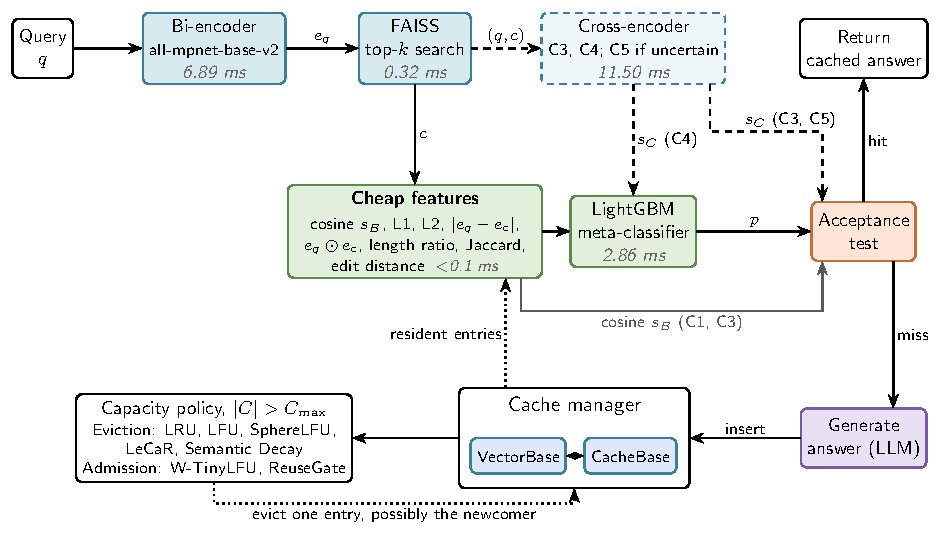
\includegraphics[width=\textwidth]{figure_1.pdf}
\caption{Semantic caching system architecture. Every request follows the decision path along the top row, annotated with the batch-size-1 cost of each stage: bi-encoder embedding, FAISS retrieval of the top-$k$ candidates, the cheap features, the LightGBM meta-classifier, and the acceptance test. The cross-encoder (dashed) scores the request--candidate pair only in the configurations that use it: its score enters the meta-classifier in C4 and the acceptance test in C3 and C5, where C5 calls it only for uncertain candidates. A miss generates a new answer and inserts it into the cache manager; when capacity binds, the capacity policy removes one entry, which for an admission policy such as W-TinyLFU or ReuseGate may be the newcomer itself.}
\label{fig:system_overview}
\end{figure*}

\subsection{Semantic Caching System Architecture}
\label{subsec:semantic_caching_architecture}

Figure~\ref{fig:system_overview} shows the two cache stores and the query path. The bi-encoder produces the reusable vectors used for retrieval, and, depending on the named configuration, the retrieved pair is accepted by a cosine threshold, a conjunction of bi-encoder and cross-encoder thresholds, or a LightGBM probability threshold \citep{ke2017lightgbm}. A miss invokes the LLM and inserts the new query, answer, and vector; a hit returns the resident answer.

\subsection{Stacking Ensemble Architecture}
\label{subsec:meta_encoder}

The stacking configurations use a learned classifier over the retrieved query--candidate pair, and the feature groups and training procedure are defined below.

\subsubsection{Feature Extraction Pipeline}
\label{subsubsec:trainable_encoder_architecture}

The stacking ensemble extracts features at three levels that capture complementary semantic information.

\textbf{Level 1: Base Model Features.}
The bi-encoder feature is the cosine similarity between 768-dimensional embeddings from \texttt{all-mpnet-base-v2}. The cross-encoder feature is the score from \texttt{cross-encoder/stsb-roberta-large}, transformed by a sigmoid function to the interval $[0,1]$.

\textbf{Level 2: Extended Embedding Features.}
When extended features are enabled, the system computes the Euclidean distance ($\lVert e_1-e_2\rVert_2$), the Manhattan distance ($\lVert e_1-e_2\rVert_1$), the element-wise product ($e_1\odot e_2$), and the absolute difference ($|e_1-e_2|$). The distance features describe overall separation, while the element-wise features retain dimension-level interactions.

\textbf{Level 3: Text-based Features.}
Surface patterns are represented by character and word counts, the query-length ratio $\min(\mathrm{len}_1,\mathrm{len}_2)/\max(\mathrm{len}_1,\mathrm{len}_2)$, Jaccard word overlap, and the normalized edit distance $d_{\mathrm{edit}}/\max(\mathrm{len}_1,\mathrm{len}_2)\in[0,1]$.


\subsubsection{Meta-Classifier Selection and Training}
\label{subsubsec:meta_classifier}
\textbf{Meta-Classifier Selection:}
Three tree ensembles are candidates for the meta-classifier: LightGBM \citep{ke2017lightgbm}, XGBoost \citep{chen2016xgboost}, and Random Forest \citep{breiman2001random}. The two gradient-boosting models reach the same F1 within one standard deviation (Section~\ref{subsubsec:individual_performance}), so the serving experiments adopt LightGBM on the basis of its batch-size-1 cost of 2.93~ms for features and inference together (Table~\ref{tab:latency_breakdown}).

For each group-disjoint fold (Section~\ref{subsec:datasets_preprocessing}), the meta-classifier is trained on the combined feature representations from the training portion and evaluated on the validation portion at a probability threshold of 0.5, the threshold that C2 applies online. The hyperparameters are fixed across folds and are not searched on the validation portions, so no classifier gains from tuning and the evaluation data do not inform the settings. All three classifiers use 400 trees. The two boosting models pair a learning rate of 0.05 with row and column subsampling of 0.9 and 0.8 and an L2 penalty of 1.0, following the practice of trading more boosting rounds for shrinkage and subsampling \citep{friedman2001greedy, friedman2002stochastic}; LightGBM uses 63 leaves with at least 20 samples per leaf and XGBoost a maximum depth of 6, while Random Forest keeps at least two samples per leaf. Reported metrics are fold means with standard deviations.


\subsection{Evaluated Cache Configurations}
\label{subsec:cache_configurations}
We evaluate five named configurations, and every reported latency, hit ratio, and token saving refers to one of these definitions.

\begin{table*}[htbp]
\centering
\caption{Components active in each evaluated configuration. All configurations use exact FAISS search over normalized bi-encoder vectors.}
\label{tab:component_activation}
\resizebox{\textwidth}{!}{
\begin{tabular}{lccccc}
\toprule
\textbf{Configuration} & \textbf{Bi-encoder} & \textbf{Cross-encoder} & \textbf{Geometric/text} & \textbf{LightGBM} & \textbf{Decision} \\
\midrule
C1: Bi-encoder only & yes & no & no & no & cosine threshold \\
C2: Cheap-feature stacking & yes & no & yes & yes & meta probability \\
C3: Cross-encoder re-ranking & yes & yes & no & no & $s_B\geq0.726$ and $s_C\geq0.557$ \\
C4: Full stacking & yes & yes & yes & yes & meta probability \\
C5: Gated verification & yes & uncertain cases & yes & yes & meta probability; $s_C\geq0.557$ inside $[0.30,0.70)$ \\
\bottomrule
\end{tabular}
}
\end{table*}

Cheap features are arithmetic over bi-encoder vectors already computed for retrieval, together with short surface-text statistics. The cross-encoder requires a second forward pass over each concatenated query pair and cannot reuse either cached embedding.

C5 follows the C2 decision outside an uncertainty band of meta-classifier probabilities: a candidate with probability of at least 0.70 is served, and one below 0.30 is rejected. Inside the band $[0.30,0.70)$ the cross-encoder decides with its own threshold, so the pairwise forward pass is paid only for uncertain candidates.

\subsection{Semantic Decay: An Exploratory Eviction Baseline}
\label{subsec:semantic_decay}
Semantic Decay tests whether semantic counterparts of recency, age, and frequency can improve eviction; it is not proposed as a final policy, and Section~\ref{subsubsec:eviction_policy_impact} shows that the room lies in admission.

Classical replacement policies rank cached entries by one of three signals: how recently an entry was requested (LRU), how long it has been resident (FIFO and expiry-based policies), and how often it has been requested (LFU). In a semantic cache, a request can be served by any entry close to it in embedding space, so each signal has a semantic counterpart that counts similar requests along with identical ones. Semantic Decay combines these counterparts into one score for each cached query $q$ at stream step $t$:
\begin{equation}
D(q,t)=w_f\,z\bigl(F(q,t)\bigr)+w_a\,z\bigl(A(q,t)\bigr)+w_b\,z\bigl(B(q,t)\bigr),
\end{equation}
where $z(\cdot)$ standardizes each component across current cache entries. Freshness $F$, the counterpart of recency, is the mean cosine similarity to the $n=20$ most recent queries. Age $A=\exp[-\gamma(t-t_0)]$ decays with the time since the insertion step $t_0$, at $\gamma=0.01$ per stream step. Boost $B$, the counterpart of frequency, is the mean cosine similarity to at most $K=20$ of the most frequently hit entries, and the entry with the lowest score is evicted. All terms use normalized bi-encoder vectors already stored in the FAISS index, so the policy performs a small matrix product only when eviction is required and never calls the cross-encoder.

The weights determine which of the three signals the policy relies on, and they are selected on a dedicated tuning stream (seed 1042), disjoint from the evaluation streams, by maximizing the correct-hit ratio averaged over capacities 300, 500 and 800 across the 21 settings of the weight simplex in steps of 0.2. The selection places all weight on the boost term, $(w_f,w_a,w_b)=(0,0,1)$, so the frequency counterpart carries the signal on this workload, consistent with LFU being the strongest classical baseline (Section~\ref{subsubsec:eviction_policy_impact}). Restricting the score to freshness and boost, the form without the age term, and selecting over eleven settings arrives at the same boost-only weights, which are held fixed throughout the evaluation.

\subsection{Evaluation Framework}
\label{subsec:evaluation_setup}
\subsubsection{Hardware and LLM Configuration}
Timing results were obtained on a single server with an NVIDIA GeForce RTX 4090 GPU and an AMD Ryzen 9 3900X CPU, using PyTorch 2.8.0 with CUDA 12.8. Online inference runs in a single process with batch size 1, and the LightGBM meta-classifier runs single-threaded; batched and concurrent costs are reported separately in Section~\ref{subsubsec:latency_breakdown}. The served LLM is \texttt{gpt-5.4-nano}, called through the OpenAI Chat Completions API between July and October 2026 with \texttt{reasoning\_effort} set to \texttt{none} and the system prompt ``You are a helpful assistant who responds briefly.'' Every distinct query in the evaluation streams was answered once, and the answer was stored together with its token counts and measured generation time. During a stream run, a miss returns the stored answer after waiting for its recorded generation time, so response times include real generation waits while every configuration receives identical answers. Threshold sweeps, eviction experiments, and other measurements of decision quality reuse cached encoder outputs and recorded generation times without waiting; their decisions do not depend on the host beyond numerical round-off, and they report no latency.

\subsubsection{Dynamic Workload}
The cache evaluation uses stateful query streams derived from QQP. Connected components of the positive QQP edges define semantic topics, and the components with more than 12 questions, which make up 0.5\% of all components but hold 4.9\% of their questions, are discarded because transitive closure over noisy labels can merge unrelated questions. Every distinct question string carries one topic label throughout a stream. Recorded negative pairs supply hard negatives, which are lexically close to an earlier query without being equivalent to it; each one is drawn from strings that have not yet appeared in the stream and belong to no positive component, so no cached answer can serve it correctly on arrival. Topic popularity follows a Zipf distribution with exponent 1.1, reflecting the skewed popularity observed in web and search-engine request streams \citep{breslau1999web,xie2002locality}.

At each step the generator emits, with probability 0.5, a repeat of an already seen topic chosen by popularity, a rate above the 31\% of similar queries reported for individual users of a chat assistant \citep{gill2024meancache}, since a shared cache collects repeats across users. A repeat uses an unseen paraphrase of the topic with probability 0.75 while one remains and an earlier string verbatim otherwise. The remaining events are hard negatives of a recent query, attempted with probability 0.35 and emitted when an unused near miss exists, or else questions from a new topic. Since about four in five QQP topics contain only two questions, paraphrases are soon exhausted, and across the five evaluation streams 40\% of requests are verbatim repeats, 10\% paraphrased repeats, 7\% hard negatives, and 43\% first occurrences of new topics. Section~\ref{subsubsec:workload_sensitivity} varies the popularity skew, repeat rate, and hard-negative rate, and Section~\ref{subsec:real_query_log} evaluates a real query log in which 52\% of queries repeat an earlier one, always as a paraphrase.

Each stream contains 2,000 requests; five independent streams generated with seeds 42 to 46 are used for evaluation, and streams generated with seeds 1042 to 1044 are reserved for tuning the capacity policies. The cache starts empty, so a first occurrence is a compulsory miss, and every miss inserts an entry, which triggers eviction when capacity binds. A hit is possible only when an equivalent query is resident at arrival time. The end-to-end and baseline runs are capacity-unbounded and never evict, while the eviction policies are evaluated under capacity pressure from 200 to 1,000 entries in Section~\ref{subsubsec:eviction_policy_impact}.

\subsubsection{Evaluation Metrics}
Each request ends in a correct hit, a false hit, or a miss. A served hit is correct when the cached entry and the request belong to the same topic, and false otherwise. Over $N$ requests with $H_c$ correct and $H_f$ false hits, the served-hit ratio $h$ and hit precision $P$ are
\begin{equation}
h=\frac{H_c+H_f}{N},\qquad P=\frac{H_c}{H_c+H_f}.
\label{eq:hit_precision}
\end{equation}
Errors are reported through the false-discovery rate (FDR) and the false-hit rate (FHR),
\begin{equation}
\mathrm{FDR}=\frac{H_f}{H_c+H_f},\qquad \mathrm{FHR}=\frac{H_f}{N},
\label{eq:false_rates}
\end{equation}
which give the share of served answers and the share of all requests that are wrong. The availability ceiling is the fraction of requests for which an equivalent entry is resident at arrival time; it bounds correct hits only, since false hits can lift the served-hit ratio above it. Correct miss measures the rejection of non-equivalent distractors. Topic labels judge whether two questions are equivalent, which does not guarantee that their answers are interchangeable, so Section~\ref{subsec:answer_audit} also audits served answers directly.

Each hit avoids one LLM call and is credited with that call's prompt and completion tokens. With $T_c$ and $T_f$ the tokens credited to correct and false hits and $T$ the tokens the stream would consume without a cache, the token saving $S$ and the correct-only saving $S_c$ are
\begin{equation}
S=\frac{T_c+T_f}{T},\qquad S_c=\frac{T_c}{T}.
\label{eq:token_saving}
\end{equation}
Neither reflects the harm of a wrong answer, which in many applications exceeds the cost of the call it replaced. We therefore charge each false hit $\lambda\geq 0$ times the tokens of that call and define the risk-adjusted saving
\begin{equation}
\mathrm{RAS}(\lambda)=\frac{T_c-\lambda\,T_f}{T}.
\label{eq:ras}
\end{equation}
A value of $\lambda=1$ corresponds to a user who simply asks again, and larger values describe applications such as customer support, finance, or healthcare, where a wrong answer carries further cost. Because $\lambda$ depends on the application, Eq.~(\ref{eq:ras}) is reported for $\lambda\in\{0,1,2,5,10\}$, together with the break-even cost
\begin{equation}
\lambda^{*}=\frac{T_c}{T_f},
\label{eq:breakeven}
\end{equation}
beyond which the cache costs more than it saves. Token metrics are reported for the same configuration and stream as response time.

Per-request timing is bounded at the point where the cache commits to a hit or a miss. That interval covers the bi-encoder forward pass, the FAISS lookup, feature extraction, and the acceptance test, and its mean is the decision overhead $\bar{o}_{\mathrm{pre}}$. A hit returns the stored answer immediately, while a miss continues into generation, insertion, and eviction. Writing $\bar{g}_{\mathrm{eff}}$ for the mean latency of that continuation over the requests a configuration missed, the mean end-to-end response time $\bar{R}$ follows
\begin{equation}
\bar{R}\approx\bar{o}_{\mathrm{pre}}+(1-h)\,\bar{g}_{\mathrm{eff}},
\label{eq:response_time}
\end{equation}
where $h$ is the served-hit ratio of Eq.~(\ref{eq:hit_precision}). The relation is approximate because a small amount of per-request bookkeeping falls outside both intervals, but across the five evaluation streams and five configurations the measured mean response time departs from Eq.~(\ref{eq:response_time}) by at most 0.27~ms, less than 0.04\% of its value. Table~\ref{tab:end_to_end} reports the measured response times.

\subsubsection{Thresholds and Similarity Search}
Individual encoders use thresholds selected on validation data by F1 maximization. C1 uses the bi-encoder threshold 0.726, C3 accepts a candidate only when the bi-encoder score is at least 0.726 and the cross-encoder score is at least 0.557, and C2 and C4 use a LightGBM probability threshold of 0.5. FAISS \citep{douze2024faiss} performs exact inner-product search over L2-normalized vectors, which is equivalent to cosine similarity. The same FAISS index and cache implementation are used for all configurations and published baselines.

\subsection{Query Processing}
For an incoming query $q$, the bi-encoder produces $e_q$ and FAISS retrieves the $k$ resident candidates with the largest cosine similarity, with $k=1$ unless stated otherwise. The active configuration scores every candidate with its decision rule: C1 applies the cosine threshold, C3 the threshold conjunction, and C2, C4, and C5 the LightGBM probability over the feature groups in Table~\ref{tab:component_activation}, computed for all candidates in one batched call. The highest-scoring accepted candidate is served and its answer returned. A miss generates and inserts a new answer and vector. If insertion exceeds $C_{\max}$, the selected capacity policy removes one entry; Semantic Decay uses the single standardized score in Section~\ref{subsec:semantic_decay}. This sequence is also the boundary used for per-request timing.

\section{Experimental Setup}
\label{sec:experiments}
This section defines the datasets, disjoint splits, model selection, and statistical procedures used by the reported experiments.


\subsection{Datasets and Preprocessing}
\label{subsec:datasets_preprocessing}
\subsubsection{Quora Question Pairs (QQP) Dataset}
QQP contains more than 400,000 question pairs across its released splits, and we use the GLUE training split, which contains 363,846 rows before cleaning. Each pair is annotated with a binary label indicating semantic equivalence: label 1 denotes semantically equivalent questions (duplicates that should result in cache hits), while label 0 denotes non-equivalent questions (unique queries requiring new LLM inference).

\textbf{Stratified Sampling Protocol:}
We first remove 559 exact repeated rows, 250 mirrored pairs, 869 self-pairs, and 35 label conflicts, which reduces the usable pool from 363,846 to 362,133 pairs. We then construct balanced subsets for individual-model and meta-classifier evaluation: the bi-encoder evaluation uses 50,000 pairs in five folds, the cross-encoder evaluation 10,000 pairs in three folds, and the meta-classifier evaluation 30,000 pairs in five folds.

QQP forms a graph because one question can appear in several pairs, so a row-level split can place the same question in both training and validation data. We form connected question components and use \texttt{StratifiedGroupKFold} to keep every component in one fold. Under ordinary stratified splitting, 27.9\% of validation questions are also present in training through another pair, and the group-disjoint protocol reduces this overlap to zero.

The cache streams are built from questions that no trained component has seen. Before any model is fitted, the connected components are partitioned into three disjoint sets, which supply the 30,000-pair meta-classifier training set, the 3,000-pair ablation subsets, and the pool from which every stream is drawn. The three sets share no component and no question string: the meta-classifier set holds 45,218 distinct questions and the ablation subsets 5,096 and 5,212, and none of them occurs among the 346,679 questions of the stream pool. The two encoder thresholds are single constants, 0.726 for the bi-encoder and 0.557 for the cross-encoder. Selecting them again on the 30,000 meta-classifier pairs, which are disjoint from the streams, gives 0.728 and 0.580 and changes the F1 score on those pairs by at most 0.0005. The pretrained encoders were not trained by us, and the pretraining corpus of the bi-encoder includes duplicate-question data from Quora, so the QQP results measure the decision layer placed on fixed encoders, and the real query log supplies the evaluation on traffic that the encoders were not trained on.

\subsubsection{STS Benchmark Validation Dataset}
We use the Semantic Textual Similarity (STS) benchmark as a secondary test of the feature-combination design \citep{cer2017semeval}. The dataset contains 8,628 sentence pairs across train (5,749), development (1,500), and test (1,379) splits; the train split is used for fitting, the development split for model selection, and the test split for the reported results. For regression, models predict the 0--5 score and are evaluated with Pearson, Spearman, and RMSE; for classification, scores of at least 2.5 are treated as similar and evaluated with F1 and AUC.

Models whose names contain ``stsb'' are excluded because they were trained on STS data. This experiment therefore uses \texttt{ms-marco-MiniLM-L-6-v2} in place of the QQP cross-encoder and tests the feature-fusion design on its own.


\subsubsection{SemBenchmarkSearchQueries Real Query Log}
\label{subsubsec:searchqueries_data}
To evaluate the configurations on real traffic, we use SemBenchmarkSearchQueries \citep{schroeder2026vcache}, a set of 150,000 search-engine queries drawn from a filtered subset of ORCAS \citep{craswell2020orcas}. Queries that yield the same response share an equivalence identifier, which the dataset authors assigned with an LLM judge. We serve the whole log, in the order of the dataset, as three consecutive streams of 50,000 queries, each starting from an empty cache. The streams hold 24,192, 24,098 and 23,970 equivalence groups, 51.6\%, 51.8\% and 52.1\% of their queries rephrase an earlier query of the same stream, and no query string recurs verbatim anywhere in the log. Since the dataset contains no responses, this evaluation reports hit ratio and precision only. The dataset carries no timestamps: its authors sampled 500,000 ORCAS queries, grouped them by $k$-means clustering of their embeddings, kept the largest clusters, and assigned equivalence identifiers within each cluster, so the row order is arbitrary and does not reproduce the order in which users asked. Section~\ref{subsubsec:leakage_controls} states how the experiments deal with this.

\subsubsection{Leakage Controls}
\label{subsubsec:leakage_controls}
Every evaluation in this paper serves real questions or real queries. The QQP streams generate the order, popularity and timing of requests from real question pairs, and the query log is served as recorded. Four rules keep evaluation data out of every fitted or tuned component.

\textit{Models trained on QQP pairs.} The meta-classifiers and the two encoder thresholds are fitted on pairs whose components, and therefore question strings, occur in no stream and in no ablation subset (Section~\ref{subsec:datasets_preprocessing}).

\textit{Settings of the capacity policies on QQP.} The weights of Semantic Decay are selected on a tuning stream (seed 1042), and the half-life and classifier of ReuseGate on tuning streams of seeds 1042 to 1044 and shifted streams built from them. ReuseGate takes its reference traffic from the streams of seeds 1045 to 1049, and all reported results use the evaluation seeds 42 to 46. All streams sample the same pool of questions independently, so they can share questions by chance: 300 of the 3,457 distinct questions of the tuning streams and 443 of the 5,758 of the reference streams also occur in the evaluation streams. No label crosses between streams, and a shared question plays the role that earlier traffic plays in a deployment, but the streams are not disjoint by topic.

\textit{The query log.} Since the log has no timestamps, ``earlier'' has no calendar meaning, and every evaluation fixes a virtual order in which the reference traffic, the tuning windows and the evaluation windows are disjoint blocks of rows, with the first two preceding the third. At arrival, a classifier sees only the request, the unlabeled reference traffic and the requests earlier in its own stream. Its training target, that a later request falls within the serving threshold, is computed inside tuning windows only. Each tuning window is scored by a model fitted on earlier tuning windows only, so no choice of threshold or of $\kappa$ uses a later window, the final model is fitted on all tuning windows, and no evaluation row enters any fit, threshold choice or statistic. Section~\ref{subsubsec:learned_admission} repeats the evaluation under three rotations of the blocks, so that every row of the log is evaluated once, and with whole topics held out of the reference and tuning data.

\textit{Reuse of rows.} The features, the LightGBM settings and the half-life of ReuseGate were fixed in preliminary experiments on rows 100,000--149,999 of the original order, with rows 50,000--99,999 serving as unlabeled reference traffic. An earlier admission policy and the decision-layer curves were evaluated on rows 0--49,999. No evaluation reported here selects anything on its own evaluation rows, but only rows 0--49,999 lay wholly outside the design of ReuseGate, so the other blocks do not count as untouched data, and we report all rotations and not only that one.

\subsubsection{QQP Subset for Latency and Ablation Analysis}
\label{subsubsec:qqp_latency_ablation_subset}
The ablation study uses a separate sample of 3,000 pairs with a 60/40 duplicate ratio, which contains 2,066 question components. Its component, question, and pair overlap with the 30,000-pair meta-classifier set is zero, and it is used only for the ablation and its linked latency comparison.

\subsection{Base Model Selection}
For the QQP stacking experiments, we select the highest-F1 bi-encoder and cross-encoder from the corresponding individual-model tables \citep{reimers2020making,gao2021simcse}.

\textbf{Bi-encoder Evaluation Results:} Table~\ref{tab:biencoder_results} presents the performance comparison of nine sentence transformer models evaluated using 5-fold cross-validation on balanced QQP subsets. All models demonstrate strong performance, with \textbf{all-mpnet-base-v2} achieving the highest F1 score of $0.836\pm0.003$ and AUC of $0.8949\pm0.0016$.

\textbf{Cross-encoder Evaluation Results:} Table~\ref{tab:crossencoder_results} shows the performance of nine cross-encoder models evaluated on the same dataset. The cross-encoders demonstrate strong performance in pairwise similarity assessment, with \textbf{cross-encoder/stsb-roberta-large} achieving the highest F1 score of $0.8286\pm0.0044$ and AUC of $0.8966\pm0.0012$. These two models supply the base scores used in the stacking configurations.

\subsection{Evaluation Metrics and Statistical Significance}
Classification is evaluated with F1 and AUC, and STS regression with Pearson correlation, Spearman correlation, and RMSE. We report fold means and standard deviations and, for the cross-encoder removal comparison, a bootstrap 95\% confidence interval over out-of-fold predictions together with a paired test.

Every model that requires normalization places \texttt{StandardScaler} as the first step of an \texttt{sklearn} pipeline fitted inside each training fold, and all reported folds are group-disjoint.

Stream results are reported as the mean over the five evaluation streams with a 95\% confidence interval from the $t$-distribution over per-stream values. Two systems are compared on the same streams with a paired $t$-test over their per-stream differences. Where a table reports a family of such comparisons, the $p$-values are adjusted with the Holm--Bonferroni procedure, and a difference is described as significant only when its adjusted $p$-value is below 0.05.


\section{Results and Analysis}
\label{subsec:main_results}

The evaluation first reports individual encoders and meta-classifiers and then examines the stateful cache, component latency, workload sensitivity, feature ablation, published baselines, answer-level correctness, encoder and index sensitivity, capacity policies, and generalization to STS and a real query log. In all tables, $\uparrow$ and $\downarrow$ mark the preferred direction and bold marks the best value within each comparison.

\begin{table}[htbp]
\centering
\caption{Bi-encoder performance on 50,000 balanced QQP pairs using five group-disjoint folds. Threshold is selected on validation data and has no preferred direction.}
\label{tab:biencoder_results}
\resizebox{\textwidth}{!}{
\begin{tabular}{lccccccc}
\toprule
\textbf{Model} & \textbf{Accuracy ($\uparrow$)} & \textbf{Precision ($\uparrow$)} & \textbf{Recall ($\uparrow$)} & \textbf{F1 ($\uparrow$)} & \textbf{AUC ($\uparrow$)} & \textbf{Threshold} \\
\midrule
\texttt{\textbf{all-mpnet-base-v2}} & \textbf{0.817 $\pm$ 0.003} & \textbf{0.759 $\pm$ 0.004} & 0.930 $\pm$ 0.005 & \textbf{0.836 $\pm$ 0.003} & \textbf{0.895 $\pm$ 0.002} & 0.726 $\pm$ 0.005 \\
\texttt{all-distilroberta-v1} & 0.810 $\pm$ 0.003 & 0.752 $\pm$ 0.004 & 0.923 $\pm$ 0.006 & 0.829 $\pm$ 0.003 & 0.884 $\pm$ 0.002 & 0.712 $\pm$ 0.004 \\
\texttt{paraphrase-MiniLM-L6-v2} & 0.798 $\pm$ 0.004 & 0.736 $\pm$ 0.007 & 0.931 $\pm$ 0.007 & 0.822 $\pm$ 0.003 & 0.873 $\pm$ 0.002 & 0.722 $\pm$ 0.007 \\
\texttt{all-MiniLM-L12-v2} & 0.791 $\pm$ 0.005 & 0.731 $\pm$ 0.009 & 0.922 $\pm$ 0.013 & 0.816 $\pm$ 0.003 & 0.873 $\pm$ 0.002 & 0.730 $\pm$ 0.011 \\
\texttt{all-MiniLM-L6-v2} & 0.790 $\pm$ 0.006 & 0.728 $\pm$ 0.011 & 0.926 $\pm$ 0.013 & 0.815 $\pm$ 0.002 & 0.873 $\pm$ 0.002 & 0.712 $\pm$ 0.015 \\
\texttt{multi-qa-MiniLM-L6-cos-v1} & 0.782 $\pm$ 0.004 & 0.718 $\pm$ 0.008 & \textbf{0.932 $\pm$ 0.015} & 0.811 $\pm$ 0.002 & 0.869 $\pm$ 0.002 & 0.696 $\pm$ 0.014 \\
\texttt{distiluse-base-multilingual-cased-v2} & 0.760 $\pm$ 0.007 & 0.699 $\pm$ 0.012 & 0.915 $\pm$ 0.017 & 0.792 $\pm$ 0.002 & 0.845 $\pm$ 0.002 & 0.716 $\pm$ 0.016 \\
\texttt{msmarco-distilbert-base-v2} & 0.755 $\pm$ 0.004 & 0.693 $\pm$ 0.007 & 0.919 $\pm$ 0.009 & 0.790 $\pm$ 0.002 & 0.842 $\pm$ 0.003 & 0.612 $\pm$ 0.012 \\
\texttt{msmarco-distilbert-base-v3} & 0.756 $\pm$ 0.003 & 0.693 $\pm$ 0.005 & 0.917 $\pm$ 0.012 & 0.790 $\pm$ 0.003 & 0.837 $\pm$ 0.002 & 0.610 $\pm$ 0.011 \\
\bottomrule
\end{tabular}
}
\end{table}


\begin{table}[htbp]
\centering
\caption{Cross-encoder performance on 10,000 balanced QQP pairs using three group-disjoint folds. Threshold is selected on validation data and has no preferred direction.}
\label{tab:crossencoder_results}
\resizebox{\textwidth}{!}{
\begin{tabular}{lccccccc}
\toprule
\textbf{Model} & \textbf{Accuracy ($\uparrow$)} & \textbf{Precision ($\uparrow$)} & \textbf{Recall ($\uparrow$)} & \textbf{F1 ($\uparrow$)} & \textbf{AUC ($\uparrow$)} & \textbf{Threshold} \\
\midrule
\texttt{\textbf{cross-encoder/stsb-roberta-large}} & \textbf{0.810 $\pm$ 0.001} & \textbf{0.756 $\pm$ 0.010} & \textbf{0.917 $\pm$ 0.025} & \textbf{0.829 $\pm$ 0.004} & \textbf{0.897 $\pm$ 0.001} & 0.557 $\pm$ 0.025 \\
\texttt{cross-encoder/stsb-roberta-base} & 0.798 $\pm$ 0.005 & 0.753 $\pm$ 0.011 & 0.889 $\pm$ 0.021 & 0.815 $\pm$ 0.006 & 0.880 $\pm$ 0.002 & 0.570 $\pm$ 0.014 \\
\texttt{cross-encoder/stsb-distilroberta-base} & 0.766 $\pm$ 0.004 & 0.709 $\pm$ 0.002 & 0.901 $\pm$ 0.013 & 0.794 $\pm$ 0.005 & 0.853 $\pm$ 0.003 & 0.530 $\pm$ 0.016 \\
\texttt{cross-encoder/stsb-TinyBERT-L-4} & 0.723 $\pm$ 0.007 & 0.666 $\pm$ 0.010 & 0.895 $\pm$ 0.021 & 0.764 $\pm$ 0.006 & 0.813 $\pm$ 0.003 & 0.513 $\pm$ 0.019 \\
\texttt{cross-encoder/ms-marco-MiniLM-L-12-v2} & 0.747 $\pm$ 0.008 & 0.690 $\pm$ 0.008 & 0.901 $\pm$ 0.001 & 0.781 $\pm$ 0.005 & 0.823 $\pm$ 0.009 & 0.110 $\pm$ 0.090 \\
\texttt{cross-encoder/ms-marco-MiniLM-L-6-v2} & 0.751 $\pm$ 0.008 & 0.703 $\pm$ 0.009 & 0.872 $\pm$ 0.004 & 0.778 $\pm$ 0.006 & 0.822 $\pm$ 0.009 & 0.150 $\pm$ 0.128 \\
\texttt{cross-encoder/ms-marco-MiniLM-L-4-v2} & 0.743 $\pm$ 0.011 & 0.708 $\pm$ 0.012 & 0.829 $\pm$ 0.005 & 0.763 $\pm$ 0.008 & 0.812 $\pm$ 0.009 & 0.113 $\pm$ 0.094 \\
\texttt{cross-encoder/ms-marco-MiniLM-L-2-v2} & 0.729 $\pm$ 0.010 & 0.706 $\pm$ 0.011 & 0.784 $\pm$ 0.005 & 0.743 $\pm$ 0.009 & 0.801 $\pm$ 0.009 & 0.073 $\pm$ 0.077 \\
\texttt{cross-encoder/ms-marco-TinyBERT-L-2-v2} & 0.725 $\pm$ 0.007 & 0.673 $\pm$ 0.007 & 0.877 $\pm$ 0.002 & 0.761 $\pm$ 0.005 & 0.794 $\pm$ 0.009 & 0.073 $\pm$ 0.104 \\
\bottomrule
\end{tabular}
}
\end{table}

\begin{table}[htbp]
\centering
\caption{Basic-feature meta-classifier performance. Results use five group-disjoint folds on 30,000 balanced QQP pairs, with normalization fitted inside each training fold.}
\label{tab:meta_classifier_basic}
\resizebox{\columnwidth}{!}{
\begin{tabular}{lccccc}
\toprule
Classifier & Accuracy ($\uparrow$) & Precision ($\uparrow$) & Recall ($\uparrow$) & F1 ($\uparrow$) & AUC ($\uparrow$) \\
\midrule
LightGBM & 0.8185 $\pm$ 0.0096 & 0.7861 $\pm$ 0.0381 & 0.8739 $\pm$ 0.0322 & 0.8267 $\pm$ 0.0169 & 0.9008 $\pm$ 0.0045 \\
XGBoost & \textbf{0.8240 $\pm$ 0.0117} & \textbf{0.7889 $\pm$ 0.0408} & \textbf{0.8838 $\pm$ 0.0291} & \textbf{0.8327 $\pm$ 0.0176} & \textbf{0.9067 $\pm$ 0.0059} \\
Random Forest & 0.8095 $\pm$ 0.0086 & 0.7846 $\pm$ 0.0377 & 0.8521 $\pm$ 0.0314 & 0.8159 $\pm$ 0.0158 & 0.8926 $\pm$ 0.0042 \\
\bottomrule
\end{tabular}}
\end{table}


\begin{table}[htbp]
\centering
\caption{Extended-feature meta-classifier performance under the same 30,000-pair group-disjoint protocol as Table~\ref{tab:meta_classifier_basic}.}
\label{tab:meta_classifier_extended}
\resizebox{\columnwidth}{!}{
\begin{tabular}{lccccc}
\toprule
Classifier & Accuracy ($\uparrow$) & Precision ($\uparrow$) & Recall ($\uparrow$) & F1 ($\uparrow$) & AUC ($\uparrow$) \\
\midrule
LightGBM & 0.8505 $\pm$ 0.0106 & \textbf{0.8457 $\pm$ 0.0142} & 0.8555 $\pm$ 0.0251 & 0.8503 $\pm$ 0.0115 & 0.9269 $\pm$ 0.0070 \\
XGBoost & \textbf{0.8522 $\pm$ 0.0123} & 0.8454 $\pm$ 0.0126 & 0.8600 $\pm$ 0.0275 & \textbf{0.8524 $\pm$ 0.0131} & \textbf{0.9273 $\pm$ 0.0069} \\
Random Forest & 0.8293 $\pm$ 0.0147 & 0.8095 $\pm$ 0.0399 & \textbf{0.8607 $\pm$ 0.0377} & 0.8331 $\pm$ 0.0199 & 0.9106 $\pm$ 0.0071 \\
\bottomrule
\end{tabular}}
\end{table}


\subsection{Individual Models and Meta-Classifiers}
\label{subsubsec:individual_performance}
Tables~\ref{tab:biencoder_results} and \ref{tab:crossencoder_results} report the individual-model baselines, and Tables~\ref{tab:meta_classifier_basic} and \ref{tab:meta_classifier_extended} report the meta-classifiers on the basic and extended feature sets. With extended features under group-disjoint five-fold evaluation, XGBoost reaches F1 $0.8524\pm0.0131$ and AUC $0.9273\pm0.0069$ and LightGBM F1 $0.8503\pm0.0115$ and AUC $0.9269\pm0.0070$, which overlap within one standard deviation, while Random Forest is lower on both; the serving experiments in the remainder of this section use LightGBM (Section~\ref{subsubsec:meta_classifier}).


\subsection{Stateful Semantic Caching Performance}
\label{subsec:stateful_cache_results}
The caching results use C2, the cross-encoder-free cheap-feature configuration, unless another configuration is named. The cache starts empty and changes after each request, and Figure~\ref{fig:dynamic_hit_ratio} follows C2 through the first 500 to 2,000 requests of each evaluation stream. The served-hit ratio rises slightly as entries accumulate, from 49.8\% to 51.3\%, and hit precision stays between 94.9\% and 95.5\%. C2 serves 97.5\% of the requests for which an equivalent entry is resident and rejects 71.5\% of the near-duplicate distractors, so its correct-hit ratio stays 1.2 to 1.3 points below the availability ceiling throughout.

\begin{figure*}[htbp]
\centering
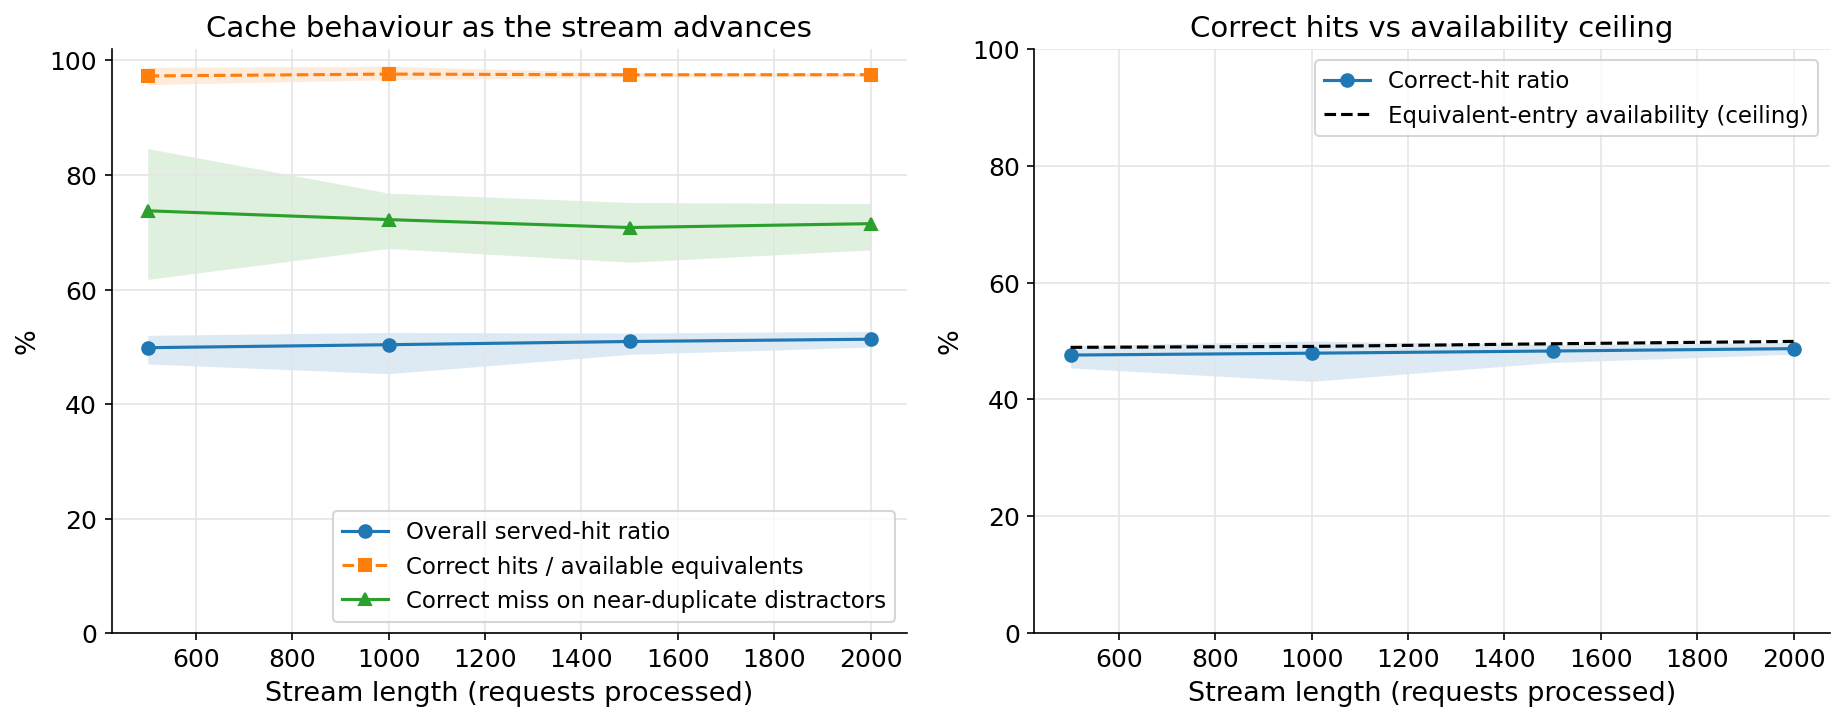
\includegraphics[width=0.92\textwidth]{fig2_dynamic_hit_ratio.png}
\caption{Dynamic cache behavior of C2 over the first 500 to 2,000 requests of the five evaluation streams; lines show the mean and shaded bands the range across streams. The left panel reports the served-hit ratio, correct hits conditional on equivalent-entry availability, and correct misses on near-duplicate distractors. The right panel places the correct-hit ratio and its availability ceiling on a 0--100\% axis.}
\label{fig:dynamic_hit_ratio}
\end{figure*}

\subsubsection{End-to-End Response Time and Token Saving}
\label{subsubsec:end_to_end}
Table~\ref{tab:end_to_end} reports the five configurations over the five evaluation streams, together with the same streams served without a cache. The decision overhead, hit statistics, response time, and token saving in each row come from the same runs, and every miss waits for the recorded generation time of its answer. Without a cache a request takes 1.87~s on average, ranging from 1.58 to 2.69~s across streams. Every configuration roughly halves this, with mean speed-ups between 2.00 and 2.13, because about half of all requests are answered from the cache within a few milliseconds. Response time therefore follows the served-hit ratio. C1, which serves the most hits, is the fastest at 0.874~s and C4 the slowest at 0.926~s; the 14.5~ms by which their decision costs differ accounts for just over a quarter of this gap, and the rest comes from the 2.2 additional points of hits served by C1. All configurations avoid 51.0--53.3\% of the tokens, of which 48.4--49.0\% are saved by correct hits.

\begin{table*}[htbp]
\centering
\caption{End-to-end results over the five evaluation streams: mean, with the 95\% $t$-interval across streams for the served-hit ratio and hit precision. Every miss waits for the recorded generation time of its answer. Decision overhead covers work up to the hit-or-miss commitment; token saving and correct-only saving follow Eq.~(\ref{eq:token_saving}).}
\label{tab:end_to_end}
\resizebox{\textwidth}{!}{
\begin{tabular}{lcccccccc}
\toprule
Configuration & Decision overhead ($\downarrow$) & Served-hit ratio ($\uparrow$) & Hit precision ($\uparrow$) & Avg.\ response ($\downarrow$) & p95 response ($\downarrow$) & Speed-up ($\uparrow$) & Token saving ($\uparrow$) & Correct-only saving ($\uparrow$) \\
\midrule
No cache & -- & -- & -- & 1.865 s & 2.62 s & 1.00$\times$ & 0.0\% & 0.0\% \\
C1: Bi-encoder only & \textbf{7.21 ms} & \textbf{53.6\% [52.5, 54.6]} & 92.2\% [90.7, 93.6] & \textbf{0.874 s} & \textbf{2.38 s} & \textbf{2.13$\times$} & \textbf{53.3\%} & \textbf{49.0\%} \\
C2: Cheap-feature stacking & 10.13 ms & 51.3\% [50.0, 52.6] & 94.9\% [94.0, 95.8] & 0.916 s & 2.39 s & 2.03$\times$ & 51.0\% & 48.4\% \\
C3: Cross-encoder re-ranking & 18.58 ms & 52.4\% [51.2, 53.6] & 93.9\% [92.7, 95.0] & 0.907 s & 2.40 s & 2.05$\times$ & 52.2\% & 48.9\% \\
C4: Full stacking & 21.66 ms & 51.4\% [50.3, 52.5] & \textbf{95.2\% [94.4, 96.0]} & 0.926 s & 2.41 s & 2.00$\times$ & 51.2\% & 48.7\% \\
C5: Gated verification & 10.70 ms & 52.1\% [51.0, 53.2] & 94.3\% [93.1, 95.5] & 0.904 s & 2.39 s & 2.06$\times$ & 51.9\% & 48.8\% \\
\bottomrule
\end{tabular}}
\end{table*}

The configurations differ mainly in how their hits divide into correct and false ones. Table~\ref{tab:c1_c2_paired} compares C1 and C2 stream by stream. C1 serves 2.25 points more hits, saves 0.63 points more tokens through correct hits, and decides 2.9~ms faster, while C2 is 2.7 points more precise. The difference originates in the near-duplicate distractors, of which C2 rejects 18.2 points more than C1, at the cost of serving 1.5 points fewer of the requests for which an equivalent entry is resident. The cheap features thus make C2 markedly more conservative on queries that are lexically close to a cached entry without being equivalent to it. Section~\ref{subsubsec:pricing_false_hits} prices this trade.

\begin{table}[htbp]
\centering
\caption{Stream-level paired comparison of C1 and C2 over the five evaluation streams: mean difference C1 $-$ C2 with its 95\% interval and paired $t$-test. All differences remain significant after Holm adjustment.}
\label{tab:c1_c2_paired}
\footnotesize
\begin{tabular}{lccc}
\toprule
Measure & $\Delta$ (C1 $-$ C2) & 95\% interval & $p$ \\
\midrule
Served-hit ratio (pp) & +2.25 & [+1.69, +2.81] & $<$0.001 \\
Hit precision (pp) & $-$2.74 & [$-$3.74, $-$1.73] & 0.002 \\
Correct miss on distractors (pp) & $-$18.16 & [$-$21.48, $-$14.84] & $<$0.001 \\
Correct hits / available equivalents (pp) & +1.46 & [+1.30, +1.62] & $<$0.001 \\
Correct-only saving (pp) & +0.63 & [+0.55, +0.71] & $<$0.001 \\
Decision overhead (ms) & $-$2.92 & [$-$2.98, $-$2.86] & $<$0.001 \\
Avg.\ response (s) & $-$0.043 & [$-$0.055, $-$0.031] & $<$0.001 \\
\bottomrule
\end{tabular}
\end{table}

\subsubsection{Latency Breakdown}
\label{subsubsec:latency_breakdown}
Table~\ref{tab:latency_breakdown} isolates the cost of each component in a test-bench setting, in which 300 batch-size-1 queries are issued against a fixed 2,000-vector index on the server described in Section~\ref{subsec:evaluation_setup}. Bi-encoding takes 6.89~ms and the FAISS lookup 0.32~ms, so the decision path of C1 costs 7.22~ms. The cross-encoder adds 11.50~ms per request and is the largest single stage, accounting for 61\% of the cost of C3 and 53\% of that of C4. Feature extraction and LightGBM inference together add 2.93~ms, of which feature computation takes less than 0.1~ms; the cheap features are therefore almost free, and their cost is essentially that of the meta-classifier. The full configuration C4 consequently costs 3.0 times as much as C1 and 2.1 times as much as C2. At their default thresholds, the 11.5~ms that C4 adds to C2 raises hit precision by 0.3 points, a difference that is not significant across the five evaluation streams (paired $t$-test, $p=0.35$).

\begin{table*}[htbp]
\centering
\caption{Fixed-index component microbenchmark: 300 batch-size-1 queries against a 2,000-vector index on the RTX 4090 server. Generation, insertion, and index growth are excluded.}
\label{tab:latency_breakdown}
\resizebox{\textwidth}{!}{
\begin{tabular}{lcccccc}
\toprule
Configuration & Bi-encoder ($\downarrow$) & FAISS ($\downarrow$) & Cross-encoder ($\downarrow$) & Features + LightGBM ($\downarrow$) & Total ($\downarrow$) & Relative to C1 \\
\midrule
C1: Bi-encoder only & 6.89 ms & 0.32 ms & -- & -- & \textbf{7.22 ms} & 1.00$\times$ \\
C2: Cheap-feature stacking & 6.89 ms & 0.32 ms & -- & 2.93 ms & 10.15 ms & 1.41$\times$ \\
C3: Cross-encoder re-ranking & 6.89 ms & 0.32 ms & 11.50 ms & -- & 18.71 ms & 2.59$\times$ \\
C4: Full stacking & 6.89 ms & 0.32 ms & 11.50 ms & 2.93 ms & 21.64 ms & 3.00$\times$ \\
\bottomrule
\end{tabular}}
\end{table*}

The stage costs account for the whole decision path in the stateful runs as well. Over the five evaluation streams, where the index grows after every miss, the mean decision overheads of C1 to C4 are 7.2, 10.1, 18.6, and 21.7~ms, within 0.15~ms of the totals in Table~\ref{tab:latency_breakdown}.

Table~\ref{tab:latency_distribution} reports the distribution of the decision-path cost. With one request in flight the distributions are narrow, and the 99th percentile stays within 1.6~ms of the mean for every configuration, but concurrency changes the picture: when 4 or 16 client threads share one serving process and GPU, requests queue behind one another, throughput stays roughly constant as clients are added, and the tail grows with the per-request cost. With 16 clients, the 95th-percentile decision time reaches 144~ms for C1, 248~ms for C2, and 487~ms for C4, and C4 serves 38 requests per second against 87 for C2. On a single serving process, the cross-encoder therefore halves the number of requests the cache can decide per second.

\begin{table*}[htbp]
\centering
\caption{Distribution of decision-path cost for single requests (batch size 1, 300 queries) and under concurrent client threads sharing one serving process and GPU. Throughput is in requests per second.}
\label{tab:latency_distribution}
\resizebox{\textwidth}{!}{
\begin{tabular}{lcccccccc}
\toprule
Configuration & Mean & p50 & p95 & p99 & p95, 4 clients & p95, 16 clients & Throughput, 1 client & Throughput, 16 clients \\
\midrule
C1: Bi-encoder only & 6.93 ms & 6.87 ms & 7.26 ms & 8.12 ms & 31.2 ms & 143.9 ms & 132 & 120 \\
C2: Cheap-feature stacking & 10.05 ms & 10.00 ms & 10.49 ms & 11.53 ms & 46.8 ms & 248.4 ms & 88 & 87 \\
C3: Cross-encoder re-ranking & 18.37 ms & 18.25 ms & 19.26 ms & 20.15 ms & -- & -- & -- & -- \\
C4: Full stacking & 21.71 ms & 21.27 ms & 22.53 ms & 23.30 ms & 94.0 ms & 486.5 ms & 45 & 38 \\
\bottomrule
\end{tabular}}
\end{table*}

Batching reduces the cost of the cross-encoder considerably (Table~\ref{tab:cross_batching}). From batch size 1 to batch size 16 the cost per pair falls by a factor of 8.5, to 1.3~ms, and it does not improve further at 32. This saving is available when many pairs are scored together, as in offline revalidation of cached entries or when several retrieved candidates of one request are scored at once (Section~\ref{subsec:topk_gating}). An online request that has a single candidate to verify cannot wait for a batch to fill, so its decision pays the batch-size-1 cost. The conclusions of this section therefore apply to online serving with one request decided at a time on the hardware described above; where the cross-encoder can be batched or runs on otherwise idle accelerator capacity, its marginal cost shrinks accordingly.

\begin{table}[htbp]
\centering
\caption{Cross-encoder cost per pair by batch size on the RTX 4090 server, timed on the cross-encoder alone over a fixed set of query pairs; at batch size 1 it is slightly below the 11.50 ms of Table~\ref{tab:latency_breakdown}, which is measured within the decision path.}
\label{tab:cross_batching}
\footnotesize
\begin{tabular}{lcccccc}
\toprule
Batch size & 1 & 2 & 4 & 8 & 16 & 32 \\
\midrule
Cost per pair & 11.00 ms & 5.80 ms & 3.04 ms & 1.70 ms & 1.29 ms & 1.37 ms \\
\bottomrule
\end{tabular}
\end{table}

\subsubsection{Pricing False Hits}
\label{subsubsec:pricing_false_hits}
Table~\ref{tab:risk_adjusted} prices the false hits of each configuration at its default threshold, averaged over the five evaluation streams. C1 serves the most correct tokens and therefore leads when a wrong answer costs nothing, but it also serves the most false hits: 7.8\% of its served answers are wrong, against 5.1\% for C2 and 4.8\% for C4. As the cost of a false hit grows, this difference comes to dominate. At $\lambda=10$ the risk-adjusted saving of Eq.~(\ref{eq:ras}) is 6.3\% for C1, 22.3\% for C2, and 23.5\% for C4, and the break-even costs of Eq.~(\ref{eq:breakeven}) are 11.9, 18.9, and 19.9. Each of C2, C3, and C4 improves on the risk-adjusted saving of C1 at every $\lambda\geq 1$ (Holm-adjusted paired $t$-tests, $p\leq 0.015$). C2 and C4 differ by at most 1.2 points, and none of these differences is significant.

\begin{table*}[htbp]
\centering
\caption{False hits and risk-adjusted saving at each configuration's default threshold, mean over the five evaluation streams. FDR and FHR follow Eq.~(\ref{eq:false_rates}), risk-adjusted saving Eq.~(\ref{eq:ras}), and the break-even cost Eq.~(\ref{eq:breakeven}).}
\label{tab:risk_adjusted}
\resizebox{\textwidth}{!}{
\begin{tabular}{lcccccccc}
\toprule
Configuration & FDR ($\downarrow$) & FHR ($\downarrow$) & $\lambda=0$ & $\lambda=1$ & $\lambda=2$ & $\lambda=5$ & $\lambda=10$ & Break-even $\lambda^{*}$ ($\uparrow$) \\
\midrule
C1: Bi-encoder only & 7.8\% & 4.20\% & \textbf{49.0\%} & 44.8\% & 40.5\% & 27.7\% & 6.3\% & 11.9 \\
C2: Cheap-feature stacking & 5.1\% & 2.62\% & 48.4\% & 45.8\% & 43.2\% & 35.4\% & 22.3\% & 18.9 \\
C3: Cross-encoder re-ranking & 6.1\% & 3.22\% & 48.9\% & 45.6\% & 42.2\% & 32.3\% & 15.8\% & 15.3 \\
C4: Full stacking & \textbf{4.8\%} & \textbf{2.47\%} & 48.7\% & \textbf{46.2\%} & \textbf{43.6\%} & \textbf{36.1\%} & \textbf{23.5\%} & \textbf{19.9} \\
\bottomrule
\end{tabular}}
\end{table*}

These differences reflect where each default threshold places a configuration on its precision--coverage curve, and every threshold can be moved. Table~\ref{tab:matched_precision} therefore compares the configurations at the same served-hit ratio, interpolating along a full threshold sweep of each stream. At 45\% and 50\% served hits the four configurations reach the same precision within 0.4 points, and no difference from C1 is significant after Holm adjustment. The cheap features and the cross-encoder thus leave the precision--coverage curve of the bi-encoder unchanged, and their default thresholds select a more conservative point on it.

\begin{table}[htbp]
\centering
\caption{Hit precision at matched served-hit ratio, mean $\pm$ standard deviation over the five evaluation streams, interpolated along each stream's full threshold sweep. No difference from C1 is significant (smallest Holm-adjusted $p=0.20$).}
\label{tab:matched_precision}
\resizebox{\columnwidth}{!}{
\begin{tabular}{lcccc}
\toprule
Served-hit ratio & C1 & C2 & C3 & C4 \\
\midrule
45\% & \textbf{99.18\% $\pm$ 0.34} & 98.81\% $\pm$ 0.51 & 98.97\% $\pm$ 0.45 & 99.01\% $\pm$ 0.41 \\
50\% & 96.32\% $\pm$ 0.97 & 96.18\% $\pm$ 1.01 & 96.21\% $\pm$ 0.81 & \textbf{96.40\% $\pm$ 1.03} \\
\bottomrule
\end{tabular}}
\end{table}

Table~\ref{tab:best_per_lambda} chooses each configuration's threshold for the false-hit cost. At its chosen threshold, C1 comes within 0.2 points of the best configuration at every cost, and no difference between configurations is significant. The choice of threshold matters far more than the choice of configuration: at $\lambda=10$, moving C1 from its default threshold to the one chosen for that cost raises its risk-adjusted saving from 6.3\% to 41.4\%, while the four configurations at their chosen thresholds lie within 1.3 points of one another. Since these thresholds are chosen on the evaluated streams, the values are an upper bound. Choosing the threshold on four streams and applying it to the fifth costs 1.3 points or less on average, so a threshold calibrated on representative traffic transfers well within a workload.

\begin{table}[htbp]
\centering
\caption{Risk-adjusted saving when each configuration's decision threshold is chosen for the false-hit cost $\lambda$ on each stream, mean over the five evaluation streams. No difference between configurations is significant (Holm-adjusted paired $t$-tests against C1).}
\label{tab:best_per_lambda}
\footnotesize
\begin{tabular}{lcccc}
\toprule
False-hit cost & C1 & C2 & C3 & C4 \\
\midrule
$\lambda=0$ & \textbf{49.2\%} & 49.1\% & 49.1\% & \textbf{49.2\%} \\
$\lambda=1$ & 46.1\% & 46.1\% & 46.1\% & \textbf{46.3\%} \\
$\lambda=2$ & \textbf{44.8\%} & 44.5\% & 44.4\% & 44.7\% \\
$\lambda=5$ & \textbf{42.7\%} & 42.0\% & 42.0\% & 42.4\% \\
$\lambda=10$ & \textbf{41.4\%} & 40.1\% & 40.2\% & 40.4\% \\
\bottomrule
\end{tabular}
\end{table}

When the cost of a wrong answer is known and labeled traffic is available, calibrating the bi-encoder threshold is therefore sufficient. When it is not, the default threshold determines the outcome, and here C2 and C4 hold up far better than C1: at $\lambda=10$ their defaults fall 17.8 and 16.9 points short of the attainable saving, compared with 35.1 points for C1, and C2 achieves this at less than half the decision cost of C4 (Section~\ref{subsubsec:latency_breakdown}). Section~\ref{subsec:topk_gating} examines two further ways of reducing false hits, abstaining near the threshold and verifying only uncertain candidates with the cross-encoder.

\subsubsection{Top-k Retrieval and Selective Verification}
\label{subsec:topk_gating}
Table~\ref{tab:topk} scores the $k$ nearest cached entries of each request and serves the best accepted candidate. Widening the candidate set leaves C1 unchanged, since its decision depends only on cosine similarity and the nearest candidate always has the highest. For the other configurations it raises the served-hit ratio by at most 0.1 points and lowers hit precision by 0.3 to 0.8 points. In this workload the additional candidates are almost never equivalent to the request, so scoring them mainly adds chances to accept a wrong one. The cost grows with $k$ for the configurations that use the cross-encoder, from 17.9 to 20.6~ms for C3, while C2 stays near 10~ms because all its candidates are scored in one LightGBM call.

\begin{table}[htbp]
\centering
\caption{Scoring the $k$ nearest cached entries and serving the best accepted candidate on the seed-42 stream. The candidates of one request are scored in a single batched call.}
\label{tab:topk}
\resizebox{\columnwidth}{!}{
\begin{tabular}{lccccc}
\toprule
Configuration & $k$ & Served-hit ratio ($\uparrow$) & Hit precision ($\uparrow$) & Correct-only saving ($\uparrow$) & Decision overhead ($\downarrow$) \\
\midrule
C1: Bi-encoder only & 1 & 53.2\% & 92.1\% & 51.3\% & 6.64 ms \\
 & 3 & 53.2\% & 92.1\% & 51.3\% & 6.73 ms \\
 & 5 & 53.2\% & 92.1\% & 51.3\% & 6.67 ms \\
 & 10 & 53.2\% & 92.1\% & 51.3\% & 6.64 ms \\
\midrule
C2: Cheap-feature stacking & 1 & 51.1\% & 94.8\% & 50.7\% & 9.54 ms \\
 & 3 & 51.1\% & 94.5\% & 50.5\% & 9.75 ms \\
 & 5 & 51.1\% & 94.5\% & 50.5\% & 9.98 ms \\
 & 10 & 51.1\% & 94.5\% & 50.5\% & 10.25 ms \\
\midrule
C3: Cross-encoder re-ranking & 1 & 51.7\% & 94.3\% & 51.0\% & 17.92 ms \\
 & 3 & 51.8\% & 93.5\% & 50.6\% & 18.78 ms \\
 & 5 & 51.8\% & 93.5\% & 50.6\% & 18.99 ms \\
 & 10 & 51.8\% & 93.5\% & 50.6\% & 20.61 ms \\
\midrule
C4: Full stacking & 1 & 51.3\% & 95.0\% & 51.1\% & 21.31 ms \\
 & 3 & 51.4\% & 94.5\% & 50.8\% & 22.31 ms \\
 & 5 & 51.4\% & 94.5\% & 50.8\% & 22.58 ms \\
 & 10 & 51.4\% & 94.5\% & 50.8\% & 24.15 ms \\
\bottomrule
\end{tabular}}
\end{table}

Selective verification targets the requests on which the meta-classifier is least certain. Table~\ref{tab:gating} varies the width of the C5 band, taking each band as the central interval that holds a given share of out-of-fold training predictions. The bands locate the meta-classifier's errors well: the narrowest holds 5\% of the training pairs but 15\% of the errors, and the widest holds 35\% of the pairs and 72\% of the errors. Passing these pairs to the cross-encoder nevertheless does not raise precision. As the band widens, C5 serves up to 1.4 points more hits and loses up to 1.8 points of precision, consistent with the cross-encoder being the weaker of the two classifiers on its own (Section~\ref{subsec:ablation}). Verification is inexpensive, since the cross-encoder is called for at most 14\% of requests and adds at most 1.7~ms, and with an empty band C5 makes exactly the decisions of C2. With the default band $[0.30,0.70)$, C5 averages 52.1\% served hits and 94.3\% precision over the five evaluation streams, against 51.3\% and 94.9\% for C2, at a decision cost of 10.7~ms.

\begin{table*}[htbp]
\centering
\caption{Selective verification and abstention on the seed-42 stream. C5 calls the cross-encoder only when the C2 probability falls inside the band, chosen on out-of-fold training predictions to hold the stated share of training pairs. Abstention treats requests within the stated margin of the threshold as misses.}
\label{tab:gating}
\resizebox{\textwidth}{!}{
\begin{tabular}{lccccc}
\toprule
Variant & Band & Cross-encoder calls per request & Served-hit ratio ($\uparrow$) & Hit precision ($\uparrow$) & Decision overhead ($\downarrow$) \\
\midrule
C2 (no verification) & -- & 0.000 & 51.1\% & 94.8\% & 9.52 ms \\
\midrule
C5: gated cross-encoder & [0.42, 0.58] (5\%) & 0.013 & 51.2\% & 94.7\% & 9.77 ms \\
C5: gated cross-encoder & [0.34, 0.66] (10\%) & 0.035 & 51.5\% & 94.7\% & 10.00 ms \\
C5: gated cross-encoder & [0.21, 0.79] (20\%) & 0.070 & 51.9\% & 93.9\% & 10.35 ms \\
C5: gated cross-encoder & [0.10, 0.90] (35\%) & 0.141 & 52.5\% & 93.0\% & 11.23 ms \\
\midrule
C2 + abstention & $\pm$0.05 around 0.5 & 0.000 & 50.8\% & 94.9\% & 9.57 ms \\
C2 + abstention & $\pm$0.1 around 0.5 & 0.000 & 50.4\% & 95.3\% & 9.57 ms \\
C2 + abstention & $\pm$0.2 around 0.5 & 0.000 & 49.5\% & 96.2\% & 9.55 ms \\
\bottomrule
\end{tabular}}
\end{table*}

Abstention sends a request to the LLM when its probability lies within a margin of the threshold. A margin of 0.2 raises hit precision from 94.8\% to 96.2\% for 1.6 points of served hits, at no additional decision cost. Since a probability below the threshold already produces a miss, abstaining within a margin $m$ is equivalent to raising the threshold to $0.5+m$, and its effect is a move along the precision--coverage curve of Section~\ref{subsubsec:pricing_false_hits}. In this workload, therefore, neither wider retrieval nor selective verification improves on C2, and the remaining lever for precision is the operating point itself.

\subsubsection{Workload Sensitivity}
\label{subsubsec:workload_sensitivity}
Table~\ref{tab:workload_sensitivity} varies one generator parameter at a time around the default stream of Section~\ref{subsec:evaluation_setup}: the Zipf exponent of topic popularity, the repeat rate, and the hard-negative rate, each over three streams. Since a hard negative is emitted only when an unused near miss exists, the table also reports the share of requests that are hard negatives. The repeat rate has by far the largest effect. Lowering it from 0.5 to 0.3 leaves fewer repeats to serve and more distractors among the requests, and precision falls to 82.2\% for C1 and 87.1\% for C2, while raising it to 0.7 lifts precision above 97\% for every configuration. The popularity skew changes neither the hit ratio nor the precision appreciably, and a higher hard-negative rate lowers precision for all configurations. The ordering of the configurations is the same in every setting, with C2 and C4 more precise than C1, and the advantage of C2 over C1 grows as the workload becomes harder: from 0.9 points at a repeat rate of 0.7 to 5.0 points at 0.3, and from 1.2 to 2.5 points as the hard-negative rate rises from 0.1 to 0.6.

\begin{table*}[htbp]
\centering
\caption{Sensitivity to workload composition: served-hit ratio / hit precision (\%), mean over three streams (seeds 42--44). One generator parameter varies at a time from the default stream (Zipf exponent 1.1, repeat rate 0.5, hard-negative rate 0.35); the hard-negative column gives the realized share of requests.}
\label{tab:workload_sensitivity}
\resizebox{\textwidth}{!}{
\begin{tabular}{lcccccc}
\toprule
Parameter & Value & Hard negatives & C1 & C2 & C3 & C4 \\
\midrule
Zipf exponent & 0.8 & 7.0\% & 54.5 / 92.1 & 52.1 / 94.4 & 53.1 / 93.9 & 52.0 / 95.1 \\
 & 1.1 (default) & 7.0\% & 53.9 / 92.6 & 51.9 / 94.8 & 52.8 / 94.1 & 52.0 / 95.4 \\
 & 1.4 & 6.2\% & 54.4 / 93.0 & 52.8 / 94.9 & 53.4 / 94.4 & 52.6 / 95.7 \\
\midrule
Repeat rate & 0.3 & 10.8\% & 36.5 / 82.2 & 33.8 / 87.1 & 34.8 / 85.8 & 33.3 / 88.6 \\
 & 0.7 & 3.5\% & 72.1 / 97.1 & 70.7 / 98.0 & 71.4 / 97.6 & 70.6 / 98.3 \\
\midrule
Hard-negative rate & 0.1 & 2.7\% & 51.4 / 95.6 & 50.0 / 96.9 & 50.6 / 96.6 & 49.9 / 97.3 \\
 & 0.6 & 9.2\% & 55.1 / 90.9 & 52.9 / 93.4 & 53.9 / 92.7 & 52.5 / 94.2 \\
\bottomrule
\end{tabular}}
\end{table*}

\subsection{Feature Group Ablation}
\label{subsec:ablation}
The ablation uses the held-out 3,000-pair subset, five group-disjoint folds, and within-fold normalization. Table~\ref{tab:ablation_isolation} evaluates the feature groups separately and Table~\ref{tab:ablation_incremental} their contribution to combined models. In isolation, the bi-encoder cosine feature alone reaches F1 $0.859\pm0.031$ at 0.006~ms, slightly above the cross-encoder score alone at $0.852\pm0.011$ and 11.498~ms.

\begin{table*}[htbp]
\centering
\caption{Feature groups in isolation on the held-out 3,000-pair QQP subset. Results use five group-disjoint folds and within-fold normalization. Marginal cost is the mean per-request stage time from the fixed-index microbenchmark of Table~\ref{tab:latency_breakdown}: feature arithmetic for the embedding-derived and text groups, and the pairwise forward pass for the cross-encoder. It excludes the shared bi-encoder forward pass and the 2.86 ms of meta-classifier inference.}
\label{tab:ablation_isolation}
\footnotesize
\begin{tabular}{lccc}
\toprule
Feature group & Number of features & F1 ($\uparrow$) & Marginal cost ($\downarrow$) \\
\midrule
Bi-encoder cosine & 1 & \textbf{0.859 $\pm$ 0.031} & \textbf{0.006 ms} \\
Cross-encoder score & 1 & 0.852 $\pm$ 0.011 & 11.498 ms \\
Distance metrics (L2, L1) & 2 & 0.847 $\pm$ 0.029 & 0.038 ms \\
Element-wise operations & 1536 & 0.849 $\pm$ 0.031 & 0.012 ms \\
Text features & 6 & 0.774 $\pm$ 0.019 & 0.019 ms \\
\bottomrule
\end{tabular}
\end{table*}

\begin{table*}[htbp]
\centering
\caption{Incremental ablation on the held-out 3,000-pair QQP subset. The first row is the bi-encoder plus cross-encoder baseline, each of the next three rows adds one feature group to it, and $\Delta$F1 is measured against that baseline. All rows use a LightGBM meta-classifier over the listed features, so the final row is a classifier trained on the cosine feature alone, which differs from the C1 threshold rule of Table~\ref{tab:latency_breakdown}.}
\label{tab:ablation_incremental}
\footnotesize
\begin{tabular}{lccc}
\toprule
Configuration & F1 ($\uparrow$) & $\Delta$F1 ($\uparrow$) & Overhead ($\downarrow$) \\
\midrule
Bi-encoder + cross-encoder & 0.8500 $\pm$ 0.0210 & +0.0000 & 21.58 ms \\
\quad with distance metrics & 0.8437 $\pm$ 0.0227 & -0.0063 & 21.61 ms \\
\quad with element-wise operations & 0.8732 $\pm$ 0.0107 & +0.0231 & 21.59 ms \\
\quad with text features & 0.8724 $\pm$ 0.0183 & +0.0223 & 21.60 ms \\
Full model & \textbf{0.8799 $\pm$ 0.0104} & \textbf{+0.0299} & 21.64 ms \\
Full model without cross-encoder & 0.8754 $\pm$ 0.0160 & +0.0254 & 10.15 ms \\
LightGBM on cosine feature only & 0.8591 $\pm$ 0.0308 & +0.0091 & \textbf{10.08 ms} \\
\bottomrule
\end{tabular}
\end{table*}
The full model reaches F1 $0.8799\pm0.0104$ and removing the cross-encoder gives $0.8754\pm0.0160$, an observed difference of 0.0045 with a bootstrap 95\% confidence interval of $[-0.0022,0.0117]$ and a paired-test $p=0.205$, so the evidence does not show a reliable cross-encoder gain on this subset.

\begin{table*}[htbp]
\centering
\caption{Accuracy gain and measured online cost. Cheap features reuse bi-encoder outputs already computed for retrieval; the cross-encoder requires a separate pairwise forward pass. $\Delta$F1 is the gain from adding a cheap group to the bi-encoder plus cross-encoder baseline of Table~\ref{tab:ablation_incremental}, and for the cross-encoder the gain from adding it to the full cheap-feature model. Added latency is the feature computation or the pairwise forward pass and excludes the 2.86 ms of meta-classifier inference shared by all stacking configurations.}
\label{tab:cheap_vs_expensive}
\footnotesize
\begin{tabular}{llcc}
\toprule
Component & Class & $\Delta$F1 ($\uparrow$) & Added latency ($\downarrow$) \\
\midrule
Element-wise operations & cheap & \textbf{+0.0231} & \textbf{0.012 ms} \\
Distance metrics & cheap & -0.0063 & 0.038 ms \\
Text features & cheap & +0.0223 & 0.019 ms \\
Cross-encoder & expensive & +0.0045 & 11.498 ms \\
\bottomrule
\end{tabular}
\end{table*}

\begin{figure}[htbp]
\centering
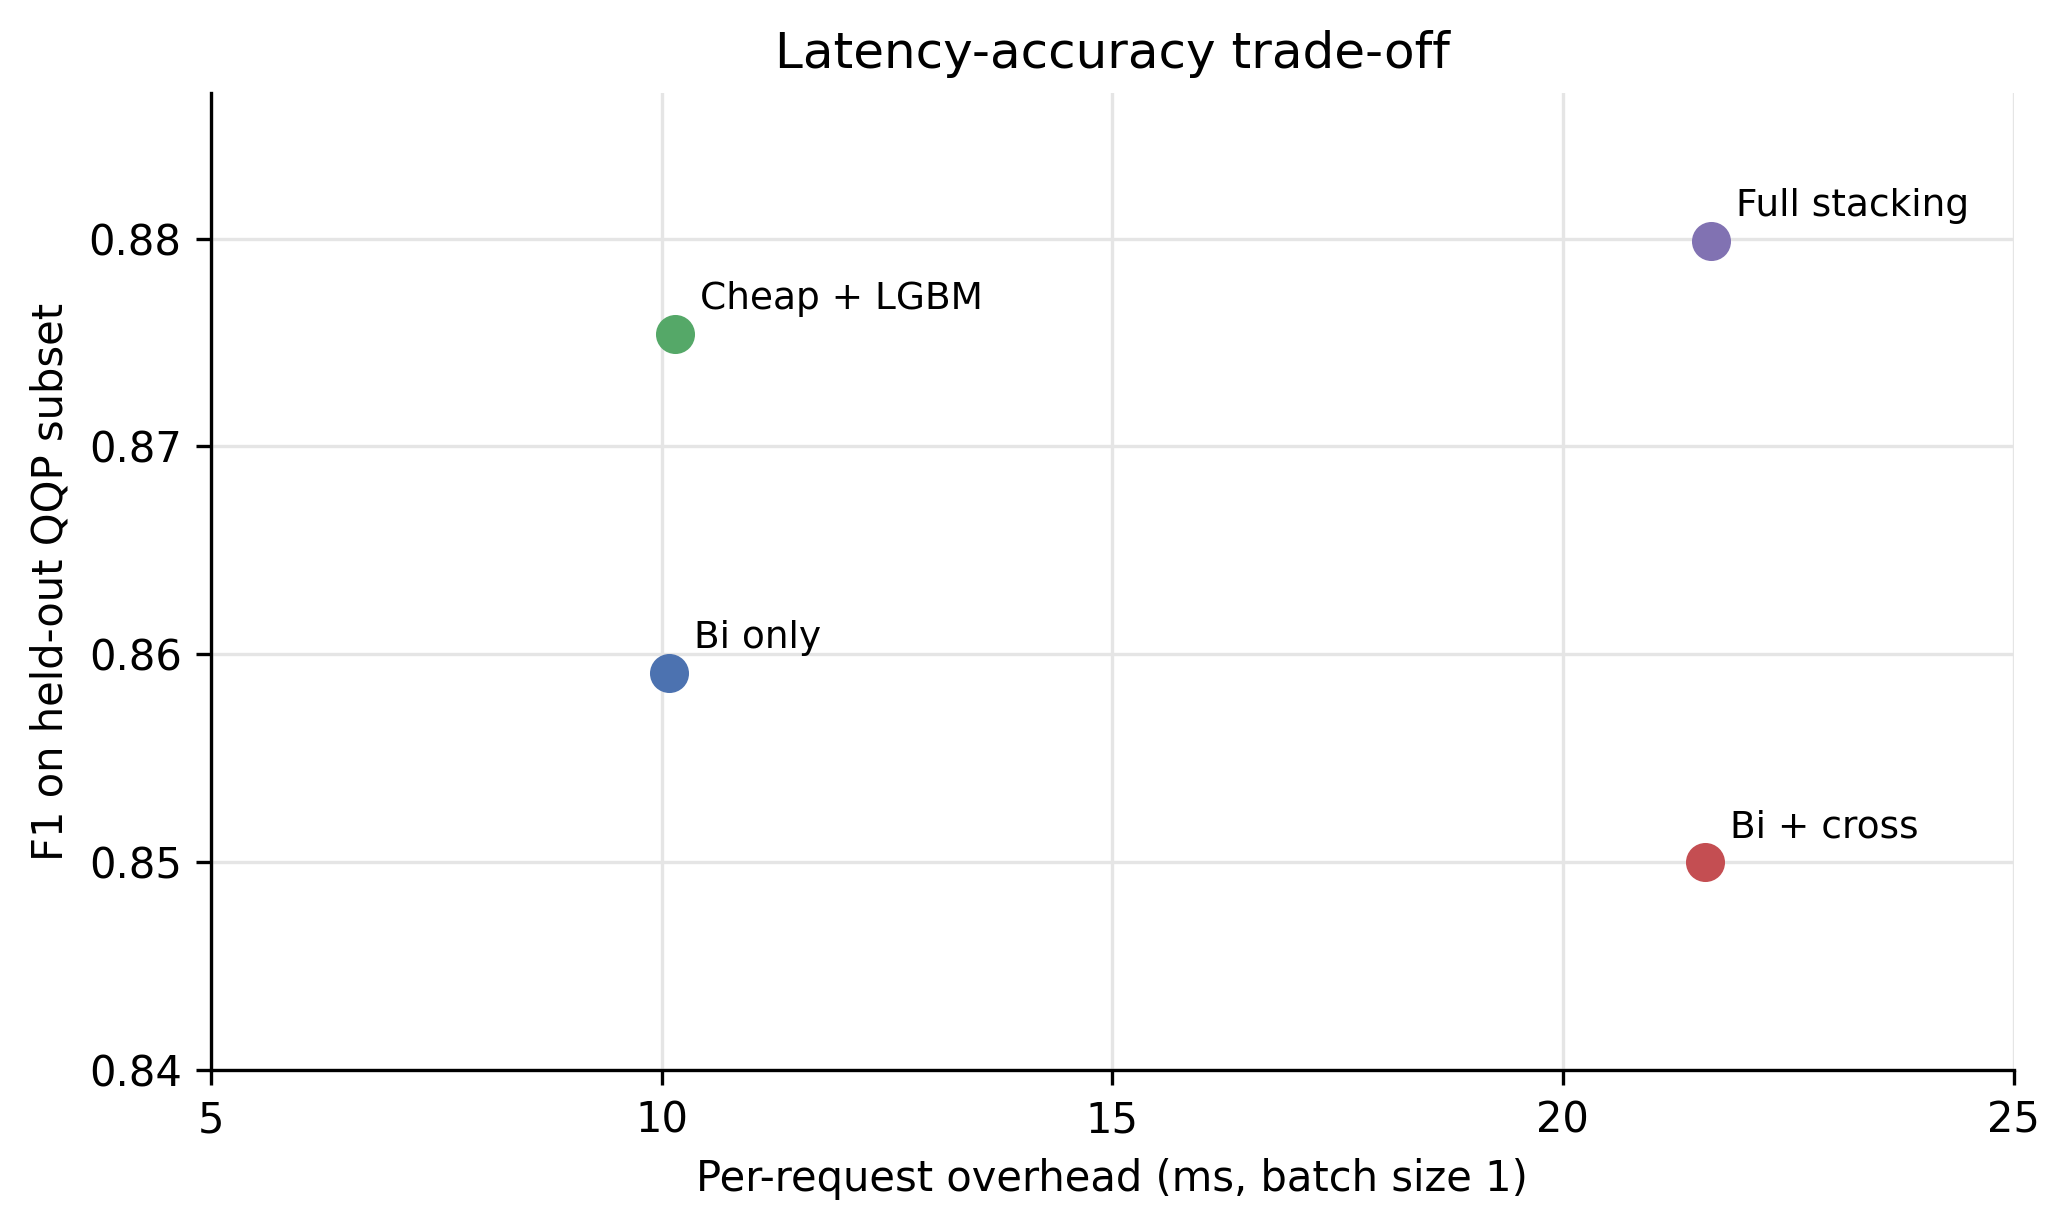
\includegraphics[width=0.95\columnwidth]{fig9_latency_accuracy_pareto.png}
\caption{F1 and batch-size-1 overhead on the held-out 3,000-pair QQP subset. Cheap-feature stacking improves the bi-encoder result with little added latency, while the cross-encoder changes the cost more than the observed F1.}
\label{fig:latency_accuracy}
\end{figure}

Cheap embedding-derived features improve F1 by 0.0163 over bi-encoder cosine at a cost of 2.93~ms relative to the classifier-free C1 path (Table~\ref{tab:latency_breakdown}), almost all of it meta-classifier inference, whereas the cross-encoder contributes 0.0045 F1 for 11.50~ms. Within the cheap group, the element-wise and text features carry the gain; adding the two distance metrics to the bi-encoder plus cross-encoder baseline reduces F1 by 0.0063, but they are retained because the group is jointly positive and their marginal cost is 0.038~ms.

\subsection{Comparison with Published Semantic Caches}
\label{subsec:baseline_comparison}
We compare against GPTCache \citep{bang2023gptcache}, SCALM \citep{li2024scalm}, VectorQ \citep{Schroeder2025VectorQ}, ContextCache \citep{Yan2025ContextCache}, and vCache \citep{schroeder2026vcache}. Each system is reimplemented at the level of its decision rule on the substrate shared by our configurations, namely the same bi-encoder, exact FAISS index, cache, streams, answers, and batch size, so that the systems differ only in how they accept a candidate and which entries they keep. GPTCache applies one global similarity threshold, and SCALM clusters cached queries and relaxes the threshold inside frequently hit clusters. VectorQ learns a threshold for each cached entry from verified feedback; our implementation receives the ground-truth label as that feedback and is therefore an upper bound on the method. ContextCache adds a context-integrated second retrieval stage, and because QQP contains no dialogues, we synthesize sessions and provide their true boundaries, which evaluates its rule on the present traffic but not on the multi-turn data for which it was designed. These four rules use the validation threshold of C1, 0.726. vCache, the later version of VectorQ, fits for each cached entry a model of the probability that a match at a given similarity is correct, and serves a hit only when the estimated error stays below a user-set bound $\delta$. It learns from a correctness check on the requests it explores, which our implementation answers with the stream labels and counts as verification calls.

Table~\ref{tab:baseline_comparison} reports the five evaluation streams. The four threshold-based rules behave almost identically to C1, serving 53.3--53.6\% hits at 92.0--92.5\% precision, and each is significantly less precise than C2, by 2.4 to 2.9 points (Holm-adjusted $p<0.03$). With C1's threshold, GPTCache applies the same decision rule as C1 and reproduces its results. Full threshold sweeps on the seed-42 stream place all four rules on the precision--coverage curve of C1, within 0.2 points at matched served-hit ratios, so their difference from C2 reflects the operating point, as it does for C1 (Section~\ref{subsubsec:pricing_false_hits}). vCache is the most precise system evaluated, at 98.5--99.5\%, but it answers only 10--28\% of requests from the cache, against 51--54\% for the threshold-based systems, and consults its correctness check on 72--90\% of requests. Its guarantee therefore trades coverage for precision, and in deployment each check must itself be paid for, through an LLM judge or user feedback.

\begin{table*}[htbp]
\centering
\caption{Published systems over the five evaluation streams: mean, with the 95\% $t$-interval across streams for the served-hit ratio and hit precision (truncated at 100\%). All systems share the bi-encoder, exact FAISS index, cache, streams, and answers. Verification calls are the correctness checks vCache requests while learning, answered here with the stream labels. C1 and C2 are repeated from Table~\ref{tab:end_to_end} for reference.}
\label{tab:baseline_comparison}
\resizebox{\textwidth}{!}{
\begin{tabular}{lccccc}
\toprule
System & Served-hit ratio ($\uparrow$) & Hit precision ($\uparrow$) & Correct-only saving ($\uparrow$) & Break-even $\lambda^{*}$ ($\uparrow$) & Verification calls per request ($\downarrow$) \\
\midrule
GPTCache & \textbf{53.6\% [52.5, 54.6]} & 92.2\% [90.7, 93.6] & \textbf{49.0\%} & 11.9 & -- \\
SCALM & \textbf{53.6\% [52.5, 54.7]} & 92.1\% [90.7, 93.6] & \textbf{49.0\%} & 11.8 & -- \\
VectorQ & 53.3\% [52.2, 54.4] & 92.5\% [91.2, 93.9] & \textbf{49.0\%} & 12.5 & -- \\
ContextCache & \textbf{53.6\% [52.5, 54.6]} & 92.0\% [90.5, 93.6] & \textbf{49.0\%} & 11.8 & -- \\
vCache ($\delta=0.01$) & 10.4\% [8.4, 12.4] & 99.1\% [97.6, 100.0] & 10.4\% & \textbf{208.4} & 0.90 \\
vCache ($\delta=0.02$) & 20.4\% [18.2, 22.6] & \textbf{99.5\% [99.1, 100.0]} & 20.2\% & 195.2 & 0.80 \\
vCache ($\delta=0.05$) & 27.6\% [24.7, 30.4] & 98.5\% [97.7, 99.3] & 26.8\% & 79.6 & 0.72 \\
\midrule
C1: Bi-encoder only & \textbf{53.6\% [52.5, 54.6]} & 92.2\% [90.7, 93.6] & \textbf{49.0\%} & 11.9 & -- \\
C2: Cheap-feature stacking & 51.3\% [50.0, 52.6] & 94.9\% [94.0, 95.8] & 48.4\% & 18.9 & -- \\
\bottomrule
\end{tabular}}
\end{table*}

\subsection{Answer-Level Audit}
\label{subsec:answer_audit}
Hit precision counts a hit as correct when the request and the cached entry belong to the same QQP topic, which tests whether two questions are equivalent. Whether the cached answer can stand in for a new one is a separate matter, which we examine with an LLM judge on the served hits of C1, C2, and C4 for the seed-42 stream. For each judged hit, the judge (\texttt{gpt-6-luna}, called through the same API in JSON mode) receives the request, the cached answer, and a reference answer freshly generated for the request by the served model, and decides whether returning the cached answer is as acceptable as generating a new one, replying with a binary verdict and a one-sentence reason. It is told that both answers were produced under the same output limit of the served model (\ref{app:judge_prompt}), so that truncation does not count against the cached answer, and that the reference indicates what the question asks without being a checklist. A cached answer is rejected only if it addresses a different question or scope, contains details that are wrong or inapplicable for the user, or omits what the user asked for.

Verbatim repeats are accepted without a call, since their answer was generated for the identical string. The remaining hits are sampled separately among label-correct and label-false hits, with up to 150 judged per stratum, which covers almost every label-false hit, and the judge-based precision reweights the two strata to each configuration's label mix.

\begin{table*}[htbp]
\centering
\caption{Answer-level audit of the served hits on the seed-42 stream. Verbatim repeats are counted as acceptable; the other hits are judged within label strata (judged pairs in parentheses), and judge-based precision reweights the strata to each configuration's label mix, with its 95\% interval.}
\label{tab:answer_audit}
\resizebox{\textwidth}{!}{
\begin{tabular}{lcccccc}
\toprule
Configuration & Served hits & Verbatim & Label precision & Judge precision ($\uparrow$) & Acceptable, label-correct & Acceptable, label-false \\
\midrule
C1: Bi-encoder only & 1065 & 413 & 92.1\% & 91.8\% [89.3, 94.3] & 92.0\% (150) & 50.6\% (83) \\
C2: Cheap-feature stacking & 1022 & 427 & 94.8\% & \textbf{96.1\% [94.4, 97.8]} & 96.6\% (148) & 58.5\% (53) \\
C4: Full stacking & 1026 & 417 & 95.0\% & 93.6\% [91.1, 96.1] & 91.8\% (147) & 60.0\% (50) \\
\bottomrule
\end{tabular}}
\end{table*}

Table~\ref{tab:answer_audit} shows that label precision is a close proxy for answer substitutability on this workload. Judge-based precision lies within 1.5 points of label precision for every configuration, and C2 reaches the highest judge-based precision, 96.1\%, although its interval overlaps that of C4. The two criteria nevertheless disagree on individual hits, and in both directions: between 51\% and 60\% of label-false hits still return an acceptable answer, while 3 to 8\% of label-correct hits do not. These disagreements largely offset, which is why the two precision measures agree. Agreement between judge and labels on individual pairs is moderate, 72.8\% (95\% bootstrap interval 67.1--78.5\%) with Cohen's $\kappa=0.40$ (0.27--0.51) over 228 judged pairs. Within the sampled strata, the judge accepts 89.8\% of label-correct and 52.7\% of label-false hits, and 71.9\% of the hits it accepts are label-correct against 24.6\% of those it rejects. These rates describe the judge within the two strata, which were sampled separately, and not the population of served hits. On individual decisions the labels and the judge therefore agree only partly. The judge instructions were settled on 30 pairs, 29 of them among these, and the other 199 give a similar agreement of 71.4\% ($\kappa=0.37$).

\subsection{Encoder and Index Sensitivity}
\label{subsec:encoder_index}
Table~\ref{tab:encoders} serves the seed-42 stream with three bi-encoders from Table~\ref{tab:biencoder_results}, each at its own validation threshold, and refits the C2 meta-classifier on the features of each encoder. The two smaller encoders roughly halve the decision cost of C1, from 6.7~ms to 3.3--3.5~ms, and serve a similar share of hits at slightly lower precision. With every encoder, C2 is more precise than C1 by 2.3 to 3.4 points and serves 2.1 to 2.6 points fewer hits, so the trade-off between the two configurations does not depend on the choice of encoder.

\begin{table}[htbp]
\centering
\caption{Bi-encoder sensitivity on the seed-42 stream. Each encoder uses its validation threshold from Table~\ref{tab:biencoder_results}, and the C2 meta-classifier is refitted on its features.}
\label{tab:encoders}
\resizebox{\columnwidth}{!}{
\begin{tabular}{lccccccc}
\toprule
 & & \multicolumn{3}{c}{C1: Bi-encoder only} & \multicolumn{3}{c}{C2: Cheap-feature stacking} \\
\cmidrule(lr){3-5}\cmidrule(lr){6-8}
Bi-encoder & Threshold & Hit ratio & Precision & Overhead & Hit ratio & Precision & Overhead \\
\midrule
all-mpnet-base-v2 & 0.726 & 53.2\% & 92.1\% & 6.71 ms & 51.1\% & \textbf{94.8\%} & 9.66 ms \\
all-distilroberta-v1 & 0.712 & 53.4\% & 91.8\% & 3.51 ms & 51.1\% & 94.1\% & 6.34 ms \\
all-MiniLM-L6-v2 & 0.712 & \textbf{54.1\%} & 90.9\% & \textbf{3.33 ms} & 51.5\% & 94.3\% & 5.11 ms \\
\bottomrule
\end{tabular}}
\end{table}

Table~\ref{tab:index} replaces exact search with HNSW ($M=32$) at efSearch values of 8, 16, and 64. HNSW cannot delete entries, so these runs use the capacity-unbounded cache of the end-to-end setting, which holds about 1,000 entries by the end of the stream. Every setting yields the same served-hit ratio and precision as exact search, and the search itself stays below 0.1~ms in all cases, under the 0.32~ms of Table~\ref{tab:latency_breakdown} because this index grows from empty to about 1,000 entries against a fixed 2,000 there; either way it is a negligible share of a decision path dominated by the encoder. At this cache size, approximate search therefore changes neither the decisions nor the cost in any material way.

\begin{table}[htbp]
\centering
\caption{Exact and approximate nearest-neighbor search (HNSW, $M=32$) on the capacity-unbounded seed-42 stream. The served-hit ratio and precision are identical for every index setting; the remaining columns give the search time per request.}
\label{tab:index}
\resizebox{\columnwidth}{!}{
\begin{tabular}{lcccccc}
\toprule
Configuration & Served-hit ratio & Hit precision & Exact & HNSW, ef 8 & HNSW, ef 16 & HNSW, ef 64 \\
\midrule
C1: Bi-encoder only & 53.25\% & 92.11\% & 0.063 ms & \textbf{0.033 ms} & 0.041 ms & 0.065 ms \\
C2: Cheap-feature stacking & 51.10\% & 94.81\% & 0.084 ms & \textbf{0.043 ms} & 0.055 ms & 0.085 ms \\
\bottomrule
\end{tabular}}
\end{table}

\subsection{Eviction Policy Evaluation}
\label{subsubsec:eviction_policy_impact}
This section evaluates Semantic Decay, which is not proposed as a deployable policy, against classical, semantic and learning-augmented eviction, and its outcome motivates the admission policy of Section~\ref{subsubsec:learned_admission}. Table~\ref{tab:semantic_decay_weights} defines the score terms, the selected weights, and the window parameters.



\begin{table}[htbp]
\centering
\caption{Semantic Decay definition used in the capacity-constrained experiments. Similarities use normalized cached bi-encoder vectors, and every score component is standardized across current cache entries. Weights are selected on the tuning stream (seed 1042).}
\label{tab:semantic_decay_weights}
\footnotesize
\begin{tabular}{llp{0.52\columnwidth}c}
\toprule
Parameter & Term & Definition & Value \\
\midrule
$w_f$ & Freshness & Mean cosine similarity to the 20-query recent window & 0 \\
$w_a$ & Age & Exponential decay from cache insertion time & 0 \\
$w_b$ & Boost & Mean cosine similarity to the 20 most frequently hit entries & 1 \\
$\gamma$ & Decay rate & $A(q,t)=\exp[-\gamma(t-t_0)]$ in stream steps & 0.01 \\
$n$ & Recent window & Number of recent queries used by Freshness & 20 \\
$K$ & Frequent set & Maximum entries used by Boost & 20 \\
\bottomrule
\end{tabular}
\end{table}

The selection surface is flat: the 21 settings span 45.7--48.1\% on the tuning stream with a standard deviation of 0.55 points, and the five best lie within 0.5 points of one another. These differences are smaller than the variation between evaluation streams, whose standard deviations range from 1.2 to 2.4 points at small capacities, so the exact optimum carries little information; what matters is which signal is present. The fourteen best settings all include the frequency counterpart, the six settings without it occupy six of the seven lowest places, and age alone gives the lowest value, 45.7\%. Recency and frequency counterparts both measure similarity to demand, and on a stationary stream the frequency signal is slightly more informative.

Capacity management is evaluated with C2 serving on the five 2,000-request evaluation streams (seeds 42--46) at capacities from 200 to 1,000 entries in steps of 100. Semantic Decay is compared with LRU, LFU, SphereLFU~\citep{biton2026spherelfu}, which spreads the frequency of each request over the cached entries inside the hit radius, and LeCaR~\citep{vietri2018lecar}, which learns online how to divide evictions between LRU and LFU from requests that return to recently evicted entries. Policies are compared by paired $t$-tests over the five streams, with Holm--Bonferroni correction across the 16 comparisons of Semantic Decay with LRU and LFU at the capacities where the policies differ.

\begin{table}[htbp]
\centering
\caption{Correct-hit ratio (\%) by cache capacity for C2 serving, mean of five evaluation streams (seeds 42--46).}
\label{tab:eviction_capacity}
\footnotesize
\setlength{\tabcolsep}{4pt}
\begin{tabular}{lccccccccc}
\toprule
Policy & 200 & 300 & 400 & 500 & 600 & 700 & 800 & 900 & 1000 \\
\midrule
LRU & 37.73 & 41.19 & 43.25 & 44.98 & 46.22 & 47.31 & 48.03 & 48.55 & 48.70 \\
LFU & \textbf{40.76} & \textbf{43.18} & \textbf{44.55} & \textbf{45.81} & 46.75 & 47.56 & 48.15 & 48.55 & 48.70 \\
SphereLFU & 39.72 & 42.41 & 44.25 & 45.55 & 46.77 & 47.59 & 48.16 & 48.55 & 48.70 \\
LeCaR & 37.80 & 41.26 & 43.26 & 44.99 & 46.23 & 47.31 & 48.04 & 48.55 & 48.70 \\
Semantic Decay & 37.10 & 41.66 & 44.08 & 45.66 & \textbf{46.84} & \textbf{47.76} & \textbf{48.25} & \textbf{48.64} & 48.70 \\
\bottomrule
\end{tabular}
\end{table}

Table~\ref{tab:eviction_capacity} reports the correct-hit ratio. Semantic Decay is not significantly better than LRU at any capacity: its difference from LRU ranges from $-0.63$ to $+0.83$ points, and no comparison remains significant after correction. It falls below LFU at small capacities, significantly so at capacity 200 ($-3.66$ points, Holm $p=0.034$). LFU gives the highest correct-hit ratio at capacities 200--500, the policies differ by less than 0.3 points from capacity 800 upward, and at 1,000 entries every policy holds the whole working set. LeCaR stays within 0.07 points of LRU at every capacity and is significantly below LFU at capacities 200--400.

To see why semantic retention gains little, Table~\ref{tab:eviction_density} records the cache contents at every eviction at capacity 400: the number of live entries within the hit radius of the victim, the share of victims whose topic is still covered by another live entry, and the share of victims that were never hit. Redundancy is low under every policy: a victim has on average 0.035--0.056 neighbors within the hit radius, and its topic remains covered in only 1.4--2.2\% of evictions. Between 82\% and 100\% of victims were never hit, so the decision that matters is which of many unrepeated entries to keep, and a score that ranks entries by their proximity to popular requests finds few near-duplicates to separate.

\begin{table}[htbp]
\centering
\caption{Cache contents at eviction time, capacity 400, C2 serving, mean of five evaluation streams. Neighbors are live entries within the hit radius of the victim; a victim's topic is covered when another live entry belongs to the same topic.}
\label{tab:eviction_density}
\footnotesize
\begin{tabular}{lccc}
\toprule
Policy & Neighbors of victim & Topic still covered (\%) & Victim never hit (\%) \\
\midrule
LRU & 0.056 & 2.25 & 82.3 \\
LFU & 0.056 & 1.91 & 100.0 \\
SphereLFU & 0.044 & 1.45 & 94.6 \\
Semantic Decay & 0.035 & 1.52 & 88.0 \\
\bottomrule
\end{tabular}
\end{table}

Weights selected once cannot follow a change in the workload, so the policies are also evaluated on five shifted streams. Each joins the first 1,000 requests of one evaluation stream to the first 1,000 of another (42$\rightarrow$43, \ldots, 46$\rightarrow$42), so that the popular topics change abruptly at the midpoint. Table~\ref{tab:eviction_shift} reports the correct-hit ratio over the second half and over the first 200 requests after the change.

\begin{table}[htbp]
\centering
\caption{Correct-hit ratio (\%) after an abrupt change of topics at request 1,000, by cache capacity, mean of five shifted streams, C2 serving. Recovery covers the first 200 requests after the change.}
\label{tab:eviction_shift}
\footnotesize
\setlength{\tabcolsep}{4pt}
\begin{tabular}{lcccccccc}
\toprule
 & \multicolumn{4}{c}{Second half} & \multicolumn{4}{c}{Recovery} \\
\cmidrule(lr){2-5}\cmidrule(lr){6-9}
Policy & 200 & 400 & 600 & 800 & 200 & 400 & 600 & 800 \\
\midrule
LRU & \textbf{42.4} & \textbf{47.2} & \textbf{48.1} & \textbf{48.2} & \textbf{44.9} & 45.1 & \textbf{45.4} & \textbf{45.4} \\
LFU & 40.0 & 45.8 & \textbf{48.1} & \textbf{48.2} & \textbf{44.9} & \textbf{45.2} & \textbf{45.4} & \textbf{45.4} \\
SphereLFU & 42.0 & 46.4 & \textbf{48.1} & \textbf{48.2} & 44.8 & 45.1 & \textbf{45.4} & \textbf{45.4} \\
LeCaR & \textbf{42.4} & \textbf{47.2} & \textbf{48.1} & \textbf{48.2} & \textbf{44.9} & 45.1 & \textbf{45.4} & \textbf{45.4} \\
Semantic Decay & 13.8 & 33.1 & 43.7 & 47.3 & 9.9 & 35.8 & \textbf{45.4} & \textbf{45.4} \\
\bottomrule
\end{tabular}
\end{table}

LRU, LeCaR and SphereLFU recover at once, and LFU trails LRU over the second half only at the two smaller capacities. Semantic Decay collapses when the cache is small. At capacity 200 it serves 13.8\% of second-half requests correctly against 42.4\% for LRU, and 9.9\% of the first 200 requests after the change against 44.9\%. Its second-half deficit remains significant at every capacity (Holm $p\le0.011$ across the eight comparisons with LRU) and shrinks from 28.5 points at capacity 200 to 0.9 points at 800. The boost term ranks entries by their similarity to the most frequently hit entries, and after a change of topics those entries belong to the old workload, so the policy keeps evicting the new topics. Because the selected score drops the recency counterpart, the one component computed from the current requests, nothing in it registers the change, much as frequency-based eviction lags recency-based eviction after a shift in classical caches. LeCaR, whose division between LRU and LFU is learned online, settles on LRU-like behavior on both kinds of stream: it matches LRU after the change and remains below LFU on stationary streams when the cache is small.

Across nine capacities and five streams, the correct-hit ratio of Semantic Decay cannot be distinguished from that of LRU, it falls below LFU when the cache is small, and its reliance on past popularity makes it fail when the popular topics change.

\subsection{ReuseGate: Learned Admission}
\label{subsubsec:learned_admission}
The low redundancy at eviction time points to a different decision. On the real query log (Section~\ref{subsubsec:searchqueries_data}), where no query repeats verbatim, a clairvoyant policy that keeps exactly the entries whose paraphrases arrive later serves 7.58\% of requests correctly under C1 at its in-domain threshold, averaged over capacities from 250 to 4,000 entries, whereas the best online policy serves 2.76\%. The clairvoyant policy gains by refusing to keep queries that are never asked again, so the room lies in admission: deciding, when a query arrives, whether it is likely to be repeated.

This decision can be learned from cheap features available at arrival. For each query we compute its length in characters and words, its digits and web tokens; the document frequency of its words in an earlier part of the traffic and their counts earlier in the stream; the number of earlier queries within cosine 0.7, 0.8 and the serving threshold, together with the highest cosine, both in that earlier traffic and earlier in the stream; and 16 principal components of its bi-encoder vector. A LightGBM classifier with fixed settings predicts whether a later request will fall within the serving threshold of the query. This target needs no annotation, since a cache observes it in its own request log. The policy, which we call ReuseGate, values each entry by the predicted probability $p$, halves positive values every $\tau$ capacities' worth of requests since the entry was last used, and evicts the entry of lowest value, the newcomer included, so a query of low predicted value is never admitted to a full cache. Where labeled traffic is available, a second variant, ReuseGate-R, trains separate classifiers for correct and false matches and values an entry at $p_{\mathrm{good}}-\kappa\,p_{\mathrm{bad}}$, never keeping an entry of negative value.

Because the log has no timestamps (Section~\ref{subsubsec:leakage_controls}), we evaluate ReuseGate in virtual orders in which disjoint blocks of rows serve, in this order, as reference traffic, tuning windows and evaluation windows. The 150,000 queries form three blocks of 50,000 rows. In rotation $r\in\{0,1,2\}$ the reference traffic, the tuning part and the evaluation part are blocks $1+r$, $2+r$ and $3+r$ (modulo three), and the tuning and evaluation parts are cut into five windows of 10,000 queries each. Over the three rotations every row of the log is evaluated exactly once, and rotation 1 evaluates rows 0--49,999, the block that lay outside the design of ReuseGate. A second protocol holds out whole topics. The queries are clustered into 30 coarse topics, the topics are divided into three groups of ten, and in each of three folds one group supplies the evaluation windows while the other two supply the reference traffic, their first 25,000 queries, and the tuning windows. A coarse cluster can cut an equivalence class, so the queries of the held-out group whose class also occurs in the other two groups are removed (12,377 to 15,134 of about 50,000 per fold). No class then spans the two sides, and each fold keeps 35,421 to 37,565 evaluation queries, in three windows of 10,000 and one window with the remainder.

For each false-hit cost $\lambda\in\{0,1,2,5,10\}$, every policy, baselines included, selects its serving threshold from $\{0.895,0.91,0.925,0.94,0.955,0.97\}$, and the learned variants also select $\kappa\in\{0,0.5,1,2,4\}$, by maximizing the correct-hit ratio minus $\lambda$ times the false-hit rate on the tuning windows. A tuning window is scored with classifiers fitted on earlier tuning windows only, so the first tuning window serves only for training, and the evaluation uses classifiers fitted on all tuning windows, with $\tau=4$. Policies are compared by paired $t$-tests over the evaluation windows, pooled over the windows of all rotations or folds, with Holm--Bonferroni correction across the five false-hit costs. The windows of one rotation share their classifier, so these tests treat the windows as more independent than they are, and we also report the gain in every rotation.

\begin{table}[htbp]
\centering
\caption{ReuseGate against classical and semantic baselines. Log columns: correct-hit ratio minus $\lambda$ times false-hit rate (\%), mean over the 15 evaluation windows of the three block rotations, which cover every row of the log once, and over capacities 250--4,000, each policy at the threshold it selects for that $\lambda$ on the tuning windows. QQP columns: correct-hit ratio and false-hit rate (\%) on streams 42--46 at capacities 200--1,000 under C2, and second-half correct-hit ratio on the five shifted streams at capacities 200--800.}
\label{tab:learned_admission}
\footnotesize
\setlength{\tabcolsep}{3.5pt}
\begin{tabular}{lccccc|ccc}
\toprule
 & \multicolumn{5}{c|}{Real query log, $\lambda$} & \multicolumn{3}{c}{QQP} \\
Policy & 0 & 1 & 2 & 5 & 10 & Correct & False & Shift \\
\midrule
LRU & 2.52 & 1.19 & 0.56 & 0.09 & $-$0.46 & 45.11 & 2.53 & \textbf{46.48} \\
LFU & 2.77 & 1.28 & 0.60 & 0.10 & $-$0.47 & 46.00 & 2.53 & 45.53 \\
SphereLFU & 2.78 & 1.28 & 0.64 & 0.11 & $-$0.52 & 45.74 & 2.52 & 46.16 \\
LeCaR & 2.52 & 1.19 & 0.56 & 0.09 & $-$0.46 & 45.13 & 2.53 & \textbf{46.48} \\
W-TinyLFU & 2.61 & 1.20 & 0.57 & 0.11 & $-$0.41 & \textbf{46.94} & 2.44 & 43.30 \\
ReuseGate & 4.44 & 2.13 & 1.10 & 0.27 & $-$0.67 & 46.81 & \textbf{2.31} & 43.02 \\
ReuseGate-R & \textbf{4.48} & \textbf{2.53} & \textbf{1.53} & \textbf{0.62} & \textbf{0.25} & -- & -- & -- \\
\bottomrule
\end{tabular}
\end{table}

Table~\ref{tab:learned_admission} reports the results. The classifier ranks the queries that will be repeated well, with an AUC of 0.845 in each of the three rotations. ReuseGate exceeds W-TinyLFU by 1.83, 0.94 and 0.54 points at $\lambda=0$, 1 and 2 (Holm $p<10^{-8}$), and exceeds LRU, LFU and SphereLFU by 0.94, 0.86 and 0.85 points at $\lambda=1$ ($p<10^{-12}$). The gain is the same in every rotation, 0.97, 0.98 and 0.85 points over W-TinyLFU at $\lambda=1$, including the rotation that evaluates the rows outside the design of ReuseGate. At $\lambda=0$ it serves 4.44\% of requests correctly against 2.61\% for W-TinyLFU. Its precision stays at the level of the baselines, 63.1\% against 62.6\%, so the false-hit rate rises with the correct hits, and its advantage narrows as false hits become costlier: it is 0.15 points ahead at $\lambda=5$ (Holm $p<0.001$) and 0.26 points behind at $\lambda=10$ ($p=0.002$). ReuseGate-R prices this risk and exceeds W-TinyLFU at every $\lambda$, by 1.88, 1.33, 0.96, 0.51 and 0.66 points (Holm $p<10^{-7}$), reaches a precision of 75.0\% at $\lambda=1$ against 67.5\% for W-TinyLFU, and is the only policy whose score stays positive at $\lambda=10$. Most of the predictive signal comes from earlier traffic: neighbor counts in the reference traffic account for 47\% of the classifier's gain, the embedding components for 28\% and term frequencies for 20\%, while counts from the current stream contribute 4\%. This explains why policies that count only the requests they have seen cannot find the queries worth keeping.

The dependence on reference traffic is limited. Without any reference traffic, the classifier sees only text, embedding and in-stream features, and its AUC falls to 0.705. ReuseGate then still exceeds W-TinyLFU by 0.70, 0.30 and 0.22 points at $\lambda=0$, 1 and 2 (Holm $p<0.001$), and LRU and LFU by 0.31 and 0.22 points at $\lambda=1$, but its advantage disappears at $\lambda=5$ ($+0.02$, $p=0.44$). With a reference of 1,000, 10,000 and 50,000 queries, the gain over W-TinyLFU at $\lambda=1$ in rotation 0 grows from 0.31 points to 0.60, 0.74 and 0.97, so a small reference already captures much of it.

The advantage also holds when the topics of the evaluation windows are absent from the reference and tuning data. In the three topic folds, ReuseGate with a reference of 25,000 queries exceeds W-TinyLFU by 0.89, 0.73 and 0.52 points at $\lambda=0$, 1 and 2 (Holm $p<0.001$) and by 0.29 points at $\lambda=5$ (Holm $p=0.027$), and exceeds LRU and LFU by 1.12 and 0.47 points at $\lambda=1$. The version without reference traffic does at least as well, with 1.16, 0.72 and 0.56 points over W-TinyLFU. Reference traffic from other topics therefore does not help: its neighbor counts describe topics to which the held-out queries do not belong, and the classifier is slightly worse with them (AUC 0.70 against 0.73). The margin over LFU depends on how the topics are partitioned. In a single split into two halves of the topics, the version with a reference exceeded LFU by 0.06 points at $\lambda=1$ ($p=0.23$), whereas the version without a reference exceeded it by 0.43 points.

On the QQP streams, where 40\% of requests repeat a query verbatim, exact-key admission already captures most of this effect. ReuseGate, trained on tuning streams 1042--1044 and three shifted streams built from them, with $\tau=2$ selected on those streams, exceeds LRU, LFU, SphereLFU and LeCaR by 0.8--1.7 points (Holm $p\le0.001$), matches W-TinyLFU, and has the lowest false-hit rate. After an abrupt change of topics, however, it trails LRU over the second half by 3.47 points (Holm $p=0.002$), as W-TinyLFU does: the value of an entry is a prediction made at its arrival, and entries of the old workload keep that value until it decays. ReuseGate therefore makes better use of a fixed capacity on stationary traffic, most of all on real paraphrase traffic, but it shares the slower adaptation of frequency-based admission when the popular topics change abruptly.

\subsection{Cross-Dataset Validation}
\label{subsec:cross_dataset_results}

\begin{table}[htbp]
\centering
\caption{Cross-encoder performance on the STS Benchmark test set ($n=1{,}379$).}
\label{tab:sts_cross_encoder_results}
\resizebox{\textwidth}{!}{
\begin{tabular}{lcccccc}
\toprule
\textbf{Model} & \textbf{Accuracy ($\uparrow$)} & \textbf{F1 ($\uparrow$)} & \textbf{AUC ($\uparrow$)} & \textbf{Pearson ($\uparrow$)} & \textbf{Spearman ($\uparrow$)} & \textbf{Samples} \\
\midrule
\textbf{cross-encoder/ms-marco-MiniLM-L-6-v2} & \textbf{0.783} & \textbf{0.807} & \textbf{0.892} & \textbf{0.809} & \textbf{0.788} & 1379 \\
cross-encoder/ms-marco-MiniLM-L-12-v2 & 0.768 & 0.798 & 0.889 & 0.806 & \textbf{0.788} & 1379 \\
cross-encoder/ms-marco-MiniLM-L-4-v2 & 0.765 & 0.789 & 0.880 & 0.791 & 0.772 & 1379 \\
cross-encoder/ms-marco-MiniLM-L-2-v2 & 0.773 & 0.789 & 0.874 & 0.779 & 0.762 & 1379 \\
cross-encoder/ms-marco-TinyBERT-L-2-v2 & 0.753 & 0.775 & 0.851 & 0.743 & 0.726 & 1379 \\
\bottomrule
\end{tabular}
}
\end{table}

\begin{table}[htbp]
\centering
\caption{Bi-encoder performance on the STS Benchmark test set ($n=1{,}379$).}
\label{tab:sts_biencoder_results}
\resizebox{\textwidth}{!}{
\begin{tabular}{lcccccc}
\toprule
\textbf{Model} & \textbf{Accuracy ($\uparrow$)} & \textbf{F1 ($\uparrow$)} & \textbf{AUC ($\uparrow$)} & \textbf{Pearson ($\uparrow$)} & \textbf{Spearman ($\uparrow$)} & \textbf{Samples} \\
\midrule
\textbf{all-mpnet-base-v2} & \textbf{0.832} & \textbf{0.833} & \textbf{0.911} & \textbf{0.840} & \textbf{0.834} & 1379 \\
all-MiniLM-L6-v2 & 0.817 & 0.818 & 0.901 & 0.827 & 0.820 & 1379 \\
distiluse-base-multilingual-cased-v2 & 0.788 & 0.798 & 0.881 & 0.817 & 0.807 & 1379 \\
msmarco-distilbert-base-v2 & 0.788 & 0.796 & 0.873 & 0.795 & 0.784 & 1379 \\
msmarco-distilbert-base-v3 & 0.785 & 0.792 & 0.872 & 0.790 & 0.781 & 1379 \\
multi-qa-MiniLM-L6-cos-v1 & 0.769 & 0.787 & 0.856 & 0.757 & 0.760 & 1379 \\
\bottomrule
\end{tabular}
}
\end{table}
The STS experiment evaluates the feature-fusion design on a second semantic-similarity dataset, using the model pool defined in Section~\ref{subsec:datasets_preprocessing}.

\subsubsection{Individual Model Baseline Performance on STS}
Tables~\ref{tab:sts_cross_encoder_results} and \ref{tab:sts_biencoder_results} report the STS test-set baselines. \texttt{all-mpnet-base-v2} reaches Pearson 0.840 and Spearman 0.834; \texttt{ms-marco-MiniLM-L-6-v2} reaches F1 0.807.

\begin{table}[htbp]
\centering
\caption{Stacking-ensemble performance on the STS Benchmark test set ($n=1{,}379$).}
\label{tab:sts_ensemble_results}
\resizebox{\textwidth}{!}{
\begin{tabular}{lcccccccc}
\toprule
\textbf{Meta-Classifier} & \textbf{Accuracy ($\uparrow$)} & \textbf{F1 ($\uparrow$)} & \textbf{AUC ($\uparrow$)} & \textbf{Precision ($\uparrow$)} & \textbf{Recall ($\uparrow$)} & \textbf{Pearson ($\uparrow$)} & \textbf{Spearman ($\uparrow$)} & \textbf{RMSE ($\downarrow$)} \\
\midrule
\textbf{LightGBM} & \textbf{0.8550} & 0.8679 & \textbf{0.9351} & 0.8854 & 0.8510 & \textbf{0.8557} & \textbf{0.8415} & \textbf{0.7976} \\
XGBoost & \textbf{0.8550} & \textbf{0.8684} & 0.9340 & 0.8824 & \textbf{0.8549} & 0.8530 & 0.8395 & 0.8044 \\
Random Forest & 0.8521 & 0.8645 & 0.9344 & \textbf{0.8869} & 0.8433 & 0.8543 & 0.8402 & 0.8021 \\
\bottomrule
\end{tabular}
}
\end{table}


\subsubsection{Ensemble Performance on STS Benchmark}
In Table~\ref{tab:sts_ensemble_results}, XGBoost has the highest binary F1 (0.8684), while LightGBM has the highest AUC (0.9351), Pearson correlation (0.8557), Spearman correlation (0.8415), and lowest RMSE (0.7976). Relative to the best bi-encoder, the LightGBM result changes F1 by +0.0349 and Pearson by +0.0157. Relative to the best cross-encoder, the changes are +0.0609 and +0.0467, so learned feature fusion carries to STS under a different cross-encoder than the QQP serving configuration. These are single test-set evaluations without fold variance, so differences of this size among meta-classifiers are not resolved.

\subsubsection{Real Query Log}
\label{subsec:real_query_log}
Table~\ref{tab:searchqueries} reports the whole search-query log of Section~\ref{subsubsec:searchqueries_data}, served as three consecutive streams of 50,000 queries with the models and thresholds trained on QQP, sweeping the thresholds of C1 and C2 to trace each operating curve. No row of the log enters any of these models. The QQP operating points do not transfer to this traffic, and the result is the same in all three streams: at their default thresholds, C1 serves 63.5--63.6\% of the queries from the cache at 41.1--41.3\% precision and C2 serves 47.4--47.6\% at 52.8--53.3\%, so more than half of the hits of C1 and nearly half of those of C2 are false. C2 remains the safer default, serving false hits on 22.2--22.5\% of queries against 37.3--37.4\% for C1, at a cost of 0.8--1.1 points of correct hits. Along the operating curves the two configurations are close, and at matched served-hit ratios C1 is 0.6 to 1.9 points more precise than C2. Precision near 70\% requires a cosine threshold of about 0.9, at which C1 serves 29.7--30.0\% of the queries. Part of the low precision is warm-up: in the first 5,000 requests of each stream the precision of C1 at its default threshold is 31\%, and it rises to 43--44\% as the cache fills. On real search traffic the operating point must therefore be calibrated on in-domain labels, and cheap features trained on another corpus do not replace that calibration.

\begin{table}[htbp]
\centering
\caption{Real query log: the three consecutive 50,000-query streams of SemBenchmarkSearchQueries, each served in log order from an empty cache with the models trained on QQP, across decision thresholds. Hit = served-hit ratio, Prec. = hit precision. Default thresholds are marked.}
\label{tab:searchqueries}
\scriptsize
\setlength{\tabcolsep}{3pt}
\begin{tabular}{llcccccc}
\toprule
 & & \multicolumn{2}{c}{Rows 0--49,999} & \multicolumn{2}{c}{Rows 50,000--99,999} & \multicolumn{2}{c}{Rows 100,000--149,999} \\
Configuration & Threshold & Hit & Prec. & Hit & Prec. & Hit & Prec. \\
\midrule
C1: Bi-encoder only & cosine $\geq 0.70$ & 67.4\% & 37.4\% & 67.5\% & 37.9\% & 67.4\% & 37.5\% \\
 & cosine $\geq 0.726$ (default) & 63.6\% & 41.1\% & 63.6\% & 41.1\% & 63.5\% & 41.3\% \\
 & cosine $\geq 0.80$ & 50.6\% & 52.3\% & 50.7\% & 51.5\% & 50.7\% & 52.3\% \\
 & cosine $\geq 0.85$ & 40.1\% & 60.8\% & 40.2\% & 60.4\% & 40.4\% & 60.8\% \\
 & cosine $\geq 0.895$ & 29.7\% & 69.0\% & 29.7\% & 69.1\% & 30.0\% & 69.6\% \\
 & cosine $\geq 0.95$ & 15.6\% & 80.7\% & 15.5\% & 80.4\% & 15.7\% & 81.7\% \\
\midrule
C2: Cheap-feature stacking & $p \geq 0.3$ & 55.4\% & 47.0\% & 55.3\% & 46.8\% & 55.4\% & 46.5\% \\
 & $p \geq 0.5$ (default) & 47.4\% & 53.3\% & 47.6\% & 52.8\% & 47.6\% & 53.1\% \\
 & $p \geq 0.7$ & 38.8\% & 60.6\% & 38.8\% & 59.9\% & 39.0\% & 60.4\% \\
 & $p \geq 0.9$ & 23.6\% & 72.4\% & 23.7\% & 72.6\% & 24.0\% & 73.0\% \\
 & $p \geq 0.97$ & 11.4\% & 83.2\% & 11.5\% & 82.1\% & 11.5\% & 82.9\% \\
\bottomrule
\end{tabular}
\end{table}

A second corpus tests the same models on another domain. SemBenchmarkLmArena \citep{schroeder2026vcache} samples 3,500 prompts from LM-Arena conversations, each of which seeds a class of up to 24 variants generated with GPT-4.1-nano, and a hit is correct when the cached prompt belongs to the class of the request. We serve its 63,796 prompts in a fixed random order from an empty cache. Its repeats are synthetic paraphrases of the seed prompts and not observed traffic, so it tests how the decision layer separates the variants of one prompt from those of others and says nothing about admission. At the QQP default thresholds C1 serves 93.5\% of the prompts at 88.9\% precision and C2 serves 91.2\% at 90.7\%, against 92.2\% and 94.9\% on the QQP streams, and at matched served-hit ratios C2 lies between 0.12 points below and 0.47 points above C1, so the two configurations again sit on one curve.

Stack Exchange is the one source of timestamped questions with human equivalence labels that we found, and it does not suit similarity caching. A question closed as a duplicate of an earlier one is equivalent in the sense that the answers of the earlier question resolve it, and its title is rarely a paraphrase. Among the oldest 20,000 questions of the gaming, Unix, Super User and Server Fault sites, the median cosine similarity between a question and the duplicate it was closed against is 0.24 to 0.55, and at a cosine of 0.895 only 0.3\% to 2.6\% of the labeled duplicate pairs are retrievable, while 6\% to 24\% of the pairs above that threshold are labeled duplicates. We therefore did not use these streams to evaluate admission. Ask Ubuntu was excluded because the transitive closure of its duplicate links merges unrelated questions into classes of thousands.

\section{Limitations and Bottlenecks}
\label{sec:limitations}
The timing results come from one GPU server with an NVIDIA GeForce RTX 4090 and an AMD Ryzen 9 3900X, serving one request at a time from a single process. Absolute costs will differ on other accelerators and serving stacks, and the value of the measurements lies in the controlled comparison among configurations on identical hardware. Under concurrency, the measured throughput and tail latency describe one serving process sharing one GPU; replicated or disaggregated deployments would change both.

The main workload is derived from QQP and contains realistic paraphrases and recorded hard negatives, but topic popularity, repeat timing and session boundaries are generated, so the cache behavior they produce is an approximation of real traffic. The search-query log provides observed repetition, but it covers one domain of short, single-turn queries. Neither workload contains natural multi-turn conversations, in which the meaning of a request depends on the turns before it and two identical strings can call for different answers. Equivalence judged on isolated queries can therefore overstate safe reuse in conversational settings, and the ContextCache comparison, which uses synthesized sessions, tests its decision rule without the dialogue structure it was designed for.

Answer substitutability is measured with one LLM judge on one stream. The judge agrees with the labels at the level of overall precision but only moderately on individual pairs, so the audit supports label precision as a workload-level proxy without validating individual decisions.

The published semantic-cache baselines share one substrate so that their decision rules can be compared directly, which improves internal fairness but does not reproduce each system's full engineering implementation. VectorQ and vCache also receive the stream labels as their correctness feedback, which makes them upper bounds on what each method achieves when that feedback must come from an LLM judge or from users. Semantic Decay is reported as an exploratory result and not as a deployable policy, since it does not improve significantly on LRU, falls below LFU at small capacities, and recovers far more slowly than LRU after abrupt topic shifts; its role in this study is to show that the room in capacity management lies in admission. ReuseGate is evaluated on one real log, a sample of one search engine's queries that carries no timestamps, so its evaluation uses virtual orders of the rows and cannot test drift over calendar time, and a second log with natural paraphrase repetition and timestamps was not available to us. Rows other than 0--49,999 were also used in the design of the method (Section~\ref{subsubsec:leakage_controls}). Its advantage depends on reference traffic: without it, the advantage over W-TinyLFU is smaller and disappears at a false-hit cost of five, and on held-out topics the margin over LFU depends on how the topics are partitioned. In label-free form, its advantage over W-TinyLFU is established for false-hit costs up to five times a correct hit and reverses at a cost of ten, and, like frequency-based admission, it adapts more slowly than LRU when the popular topics change abruptly.

Finally, a shared cache can expose information across users. A response generated for one user may contain personal or context-specific content that should not be served to another, and a cache hit itself can reveal that a similar query was asked before. Deployments serving several users should therefore partition caches by user or tenant where answers may be personalized, restrict caching to responses free of personal content, and apply retention limits and access control, or adopt local and federated designs \citep{kim2025overview,li2025survey}.

\section{Conclusion and Future Work}
\label{sec:conclusion}
This study evaluates semantic caching as a stateful system, measuring five configurations under one online protocol on QQP-derived streams and a real search-query log. The cross-encoder is the most expensive stage of the decision path, adding 11.5~ms per request on a GPU server, yet it raises F1 by an amount that is not statistically significant and, at the default thresholds, raises hit precision by 0.3 points without significance. In end-to-end serving on the QQP streams, every configuration roughly halves response time, with speed-ups of 2.00 to 2.13, and avoids 51--53\% of the tokens, 48--49\% through correct hits, so on the default online path the cross-encoder adds cost without a measurable return.

The configurations differ mainly in how their hits divide into correct and false ones, and pricing false hits makes this difference explicit. Every configuration and every reimplemented published rule lies on the precision--coverage curve of the bi-encoder, so the operating point matters more than the configuration. When the cost of a wrong answer is known and labeled traffic is available, calibrating the bi-encoder threshold suffices. When it is not, the cheap-feature configuration C2 is the safest default: at a false-hit cost of 10 its default threshold falls 17.8 points short of the attainable saving against 35.1 points for the bi-encoder alone, at less than half the decision cost of the full model. An LLM judge confirms that label precision tracks answer substitutability on this workload within 1.5 points. The same holds on real search traffic, where C1 and C2 lie within 1.9 points of each other along their operating curves in all three streams of the log, and in a second domain within half a point, and the threshold must be calibrated on in-domain labels, so the threshold-centered view carries over from the benchmark to observed queries.

For capacity management, semantic eviction does not improve significantly on LRU, and the low redundancy of a capacity-limited cache points toward admission. ReuseGate, a learned policy that predicts from cheap features whether an arriving query will be repeated, is the capacity-management contribution: it serves 1.6 times as many correct hits as the best baseline on the real log, in every rotation of the log and, by a smaller margin, without reference traffic and on topics absent from its training data. It remains ahead when false hits cost up to five times a correct hit, and at every cost when labeled traffic is available. Like frequency-based admission, it recovers more slowly than LRU after an abrupt change of topics.

Future work should evaluate natural multi-turn conversations and production traces from several domains, examine cross-user isolation of cached responses, and measure the decision path on other serving hardware.
\appendix
\section{Judge Prompt}
\label{app:judge_prompt}
The answer-level audit of Section~\ref{subsec:answer_audit} sends each judged pair to \texttt{gpt-6-luna} as one system message and one user message. The system message is identical for every pair:
\begin{lstlisting}[basicstyle=\linespread{1.1}\footnotesize\ttfamily, columns=fullflexible, breaklines=true, breakatwhitespace=true, breakindent=0pt, frame=single, framesep=4pt, xleftmargin=4pt, xrightmargin=4pt]
You evaluate a semantic cache for a question-answering assistant. A user asked a question. The cache returned an answer that was originally generated for a different but similar question. Decide whether giving the user the cached answer is as acceptable as generating a new answer for their question.

Both answers were produced under the same output limit of 256 tokens, so either may stop mid-sentence. Do not count truncation against the cached answer.

A reference answer generated for the user's question is provided as a guide to what the question asks. It is not a checklist: the cached answer need not cover the same points or match its wording.

Answer not_substitutable only if the cached answer (a) addresses a different question or a different scope than the user asked about, (b) contains content that is wrong or inapplicable for this user, for example details tied to a person, place, quantity or condition that differs from the user's question, or (c) omits the specific thing the user asked for. Otherwise answer substitutable.

Reply with JSON only: {"verdict": "substitutable" | "not_substitutable", "reason": "<one sentence>"}
\end{lstlisting}
The user message fills the request, the cached answer, and the reference answer into the following template:
\par\noindent\begin{minipage}{\linewidth}
\begin{lstlisting}[basicstyle=\linespread{1.1}\footnotesize\ttfamily, columns=fullflexible, breaklines=true, breakatwhitespace=true, breakindent=0pt, frame=single, framesep=4pt, xleftmargin=4pt, xrightmargin=4pt]
User question:
{request}

Cached answer (returned to the user):
{cached answer}

Reference answer for the user's question:
{reference answer}
\end{lstlisting}
\end{minipage}

% \bibliography{sn-bibliography}% common bib file
%% if required, the content of .bbl file can be included here once bbl is generated
%%\input sn-article.bbl
%\bibliographystyle{elsarticle-num} 
\renewcommand{\bibfont}{\small}
\bibliographystyle{elsarticle-harv}
\bibliography{sn-bibliography}


\end{document}
